\documentclass[titlepage,openright,letterpaper,12pt]{book}
\usepackage{entete,commandes} % Load les packages et définit des commandes.

%=============================================================================%

% On crée des bools qui sont False par défaut.
\newtoggle{VersionLivre}
\newtoggle{LivrePGChVide}
\newtoggle{ForceEntete}
\newtoggle{AuteureFemme}
\newtoggle{MemoirePasThese}
\newtoggle{useCustomFonts}
\newtoggle{generatePDFa}
\newtoggle{IntroConcluSansNombre}

% Switchboard, l'endroit ou on ajuste les toggles.
% Décommenté -> True; commenté -> False

%\toggletrue{VersionLivre}          % Décommenter pour faire la version livre
%\toggletrue{LivrePGChVide}         % Page gauche de chapiter vide en mode livre.
%\toggletrue{ForceEntete}            % Entête même pour version électronique.
%\toggletrue{AuteureFemme}          % Décommenter si l'auteur est une femme.
\toggletrue{MemoirePasThese}       % Décommenter dans le cas d'un mémoire.
\toggletrue{IntroConcluSansNombre}  % Intro et conclusion non numérotées
\toggletrue{useCustomFonts}         % Fonts différents, voir switchboard.tex.
%\toggletrue{generatePDFa}           % Génère un PDFa plutôt qu'un PDF standard.

%=============================================================================%

\title          {Énumération combinatoire avec les algorithmes variationnels quantiques} % Pour la page de titre/jury.
% Titre alternatif: Échantillonage et comptage avec les algorithmes variationnels quantiques
\author         {Julien Drapeau}  % Idem
\Organisation   {UNIVERSITÉ de SHERBROOKE}
\Location       {Sherbrooke, Québec, Canada}
\ResumeCourt    {On présente des résultats nouveaux dans un domaine en pleine effervescence.}
\date           {\today}       % Idem
\MotsClefs      {Mots-Clefs \sep Pertinents \sep avec séparateurs}

% On cache le code exécuté dans ce fichier parce qu'il est laid et impertinent.
\input{switchboard.tex}

%=============================================================================%

\begin{document}

%=============================================================================%
% Titre
\input{titlepage.tex}

\frontmatter % Pagination de préambule

% Jury
\begin{comment}
\end{comment}
\makeatletter   % Permet d'accèder aux variables @

\iftoggle{LivrePGChVide}
{}
{
    % Next two lines force a linebreak in ebook versions
    \chapter*{}
    \vspace{-4.7cm}
}

\thispagestyle{empty}

\begin{center}
    \vglue 2cm
    Le 10 mai 2025 \\ 
    %Le \@date % Lorsque le document sera accepté!
    \vspace{2cm}
    \scalebox{1} % Empêche le retour à la ligne si le nom est trop long.
    {\it le jury a accepté \leDocument\ de \monsieurMadame~\@author~dans sa version finale.} 
    
    \vspace{2cm}
    Membres du jury\\
    \vspace{2cm}

    Professeur Stefanos Kourtis\\
    Directeur de recherche\\
    Département de physique\\
    \vspace{2cm}
    
    Professeur André-Marie Tremblay\\
    Membre interne\\
    Département de physique\\
    \vspace{2cm}

    Professeur Baptiste Royer\\
    Président rapporteur\\
    Département de physique\\
    \vspace{2cm}
\end{center}

%\clearpage

\makeatother    % Plus d'accès aux variables @


% Dédicace
\begin{comment}
\end{comment}

\chapter*{}
\vspace{-10pt}
\setlength\epigraphwidth{.5\textwidth}
\setlength\epigraphrule{0\textwidth}
\epigraph{« Je vis parce que les montagnes ne savent pas rire, ni les vers de terre chanter. »}{- Emil Cioran}
\thispagestyle{empty}

% Sommaire
\clearpage % Mets le sommaire à la bonne page dans la TOC
\chapter*{Sommaire}
\addcontentsline{toc}{chapter}{Sommaire}
En exploitant à la fois les ressources classiques et quantiques, les algorithmes variationnels quantiques peuvent exécuter des tâches computationnelles complexes sur des ordinateurs quantiques bruités, sans nécessiter de correction d'erreurs. Ces algorithmes visent notamment à résoudre des problèmes d'optimisation combinatoire, se plaçant ainsi en concurrence avec des algorithmes classiques perfectionnés au fil des décennies. Une approche complémentaire consiste à se tourner vers des problèmes intrinsèquement plus complexes: les problèmes de comptage. Ces derniers, qui consistent à déterminer le nombre de solutions aux problèmes de décision, pourraient se révéler plus accessibles aux algorithmes variationnels quantiques qu'aux algorithmes classiques. 

Dans le cadre de ce mémoire, un algorithme surnommé VQCount est introduit pour la résolution de problèmes de comptage. VQCount s'appuie sur l'équivalence entre l'échantillonnage aléatoire et le comptage approximatif pour estimer le nombre de solutions à un facteur multiplicatif près, en exploitant l'ansatz quantique à opérateurs alternants comme générateur de solutions. Cette approche nécessite un nombre d'échantillons polynomial selon la taille du problème même lorsque ce dernier possède un nombre exponentiel de solutions, une amélioration exponentielle par rapport à des travaux précédents. 

À l'aide de simulations de réseaux de tenseurs, la performance de VQCount avec des circuits de faible profondeur est étudiée sur des instances synthétiques de deux problèmes \textsf{\#P}-difficile, positif \#1-in-3SAT et positif \#NAE3SAT, en employant comme générateurs de solutions l'algorithme quantique d'optimisation approximative ainsi que l'ansatz quantique à opérateurs alternants avec forçage de Grover. Un compromis entre la probabilité de succès et l'uniformité de l'échantillonnage du générateur est observé et exploité pour atteindre un gain en efficacité exponentiel par rapport à l'échantillonnage par rejet naïf. Ces résultats obtenus soulignent le potentiel et les limitations des algorithmes variationnels quantiques pour le comptage approximatif.

\noindent
\textbf{Mots-clés:} Algorithmes variationnels quantiques, Échantillonnage aléatoire, Comptage approximatif, Auto-réductibilité, Satisfaisabilité, Réseaux de tenseurs

% Remerciements
\chapter*{Remerciements}
\begin{comment}
\end{comment}

Ces dernières furent parfois exilarante, parfois éprouvante, mais j'en ressors indubitablement grandit. J'ose espérer que mon parcours ne s'arrête pas là, et que j'aurais l'occasion d'en apprendre davantage et d'améliorer la personne que je suis.

À ma mère et mes soeurs, pour leur soutien infaillible

À Justin, Léanne, Thibault, Thomas, Philippe et William, j'apprécie énormément votre présence à mes côtés. Vous ne cessez de 

À Antoine, Benjamin, Jérémie, Martin, Pierre-Alexandre et tous les membres du groupe, merci d'alléger le poids des études académiques

À Sovannie, merci de m'avoir fait ressentir l'intensité de la vie, avec ses hauts et ses bas. Merci de m'avoir fait découvrir à nouveau la beauté de la connexion humaine.

À Stefanos, pour avoir été un superviseur de recherche irréprochable durant mon parcours académique. Merci de m'avoir fait découvrir un domaine de recherche passiannantg  



% Tables des matières/Figures
{
    \setlength{\parskip}{0ex}
    \tableofcontents
    \listoffigures
    %\listoftables
}

%=============================================================================%

\mainmatter % Pagination standard
\onehalfspacing

%-----------------------------------------------------------------------------%

% \include serait préférable à \input à partir d'ici, mais MiKTeX sur Windows
% n'aime pas les \cite dans un \include. Fonctionne parfaitement sur TeXLive.

\begin{comment}
\end{comment}

\Introduction   % Chapitre qui ne sera pas numéroté si IntroConcluSansNombre est Vrai

%-----------------------------------------------------------------------------%

\textcolor{mydarkred}{\textit{It is currently unknwon wheter quantum computing can provide an advantage over classical algorithms}}







Le travail effectué au cours de ce projet a mené à la publication d'un article scientifique sur \textit{ArXiV}:

\textcolor{mydarkred}{\textit{Rajouter le lien.}}

Ce mémoire prend ainsi son inspiration de cet écrit.

\begin{comment}
Problème NP vs #P
Théorème de Toda
Description du paper JVV
Complexité exacte vs approximative
Countage exact vs approximatif
Borne sur le comptage ("a tighter bound for counting max-weight solutions to 2SAT instances" ou l'équivalent pour 3SAT)
\end{comment}

\chapter{Complexité du comptage}
\label{cha:complexite-du-comptage}

\begin{comment}
    \subsection*{Plan}
    
    \begin{enumerate}
        \item Introduire les problèmes algorithmiques difficiles
        \item Décrire les applications de ces problèmes
        \item Expliquer les prochaines sections
        \item Expliquer pourquoi on ne parle pas des machines de Turing (thèse de Church-Turing)
    \end{enumerate}
\end{comment}

Les problèmes de comptage surgissent dans de nombreuses disciplines, avec des applications en raisonnement probabiliste~\cite{rothHardnessApproximateReasoning1996, sangPerformingBayesianInference2005, abramsonHailfinderBayesianSystem1996}, en fiabilité des réseaux~\cite{valiantComplexityEnumerationReliability1979, duenas-osorioCountingBasedReliabilityEstimation2017}, en mécanique statistique~\cite{jerrumPolynomialtimeApproximationAlgorithms1993} et en intelligence artificielle~\cite{balutaQuantitativeVerificationNeural2019}.

Il est souvent favorable de décrire la théorie de la complexité à l'aide du concept de \textit{machine de Turing}. Cependant, ce mémoire suppose que la thèse de Church-Turing soit vraie, et donc que n'importe quel modèle de calcul puisse être utilisé de manière équivalente, pour faire abstraction de ce langage et simplifier les idées présentées.

%-----------------------------------------------------------------------------%

\section{Classes de complexité}

\begin{comment}
\subsection*{Plan}

\begin{enumerate}
    \item Définir comment quantifier la complexité d'un problème (temps contre espace)
    \item Décrire le but des classes de complexité
    \item Expliquer les propriétés des classes de complexité et leurs relations
    \item Expliquer la notation de la complexité (O notation) et les machines de Turing
    \item Décrire la tour de complexité (hiérarchie polynomiale) 
    \item Comparer les classes importantes: P et NP et \#P
    \item Établir la conjecture P != NP
    \item Mentionner le théorème de Toda
    \item Parler des classes de complexités quantique
    \item Parler de la these de church-turing pour les ordis quantiques
\end{enumerate}

\subsection*{Références}

1. Moore, Cristopher, and Stephan Mertens, The Nature of Computation (Oxford, 2011; online edn, Oxford Academic, 17 Dec. 2013), https://doi.org/10.1093/acprof:oso/9780199233212.001.0001, accessed 19 July 2024.

2. Arora, S. and Barak, B. Computational Complexity: A Modern Approach. (Cambridge University Press, Cambridge, 2009). doi:10.1017/CBO9780511804090.
\end{comment}

La théorie de la complexité s'intéresse à la classification des problèmes algorithmiques en \textit{classes de complexité}, c'est-à-dire en ensembles de problèmes de même complexité. Classifier un problème permet de caractériser les ressources nécessaires pour sa résolution par un algorithme. Les problèmes d'une même classe possèdent une difficulté inhérente similaire, ce qui permet le choix d'un algorithme et de ressources appropriées en conséquence. Savoir qu'un problème n'est pas réalistement résoluble, ou plus précisément intraitable, limite les attentes. Sachant ceci, la recherche dans cette direction peut s'avérer grandement utile. La théorie de la complexité cherche aussi à comparer les problèmes de différentes complexités. Ces comparaisons permettent de comprendre l'espace des problèmes en plus grande profondeur. Par exemple, il est évident que certains problèmes sont plus facile à résoudre que d'autres. Comparer des problèmes faciles avec des problèmes difficiles peut aider à comprendre ce qui rend un problème difficile et donc à trouver des algorithmes résolvant efficacement les problèmes plus complexes. Des liens, nommés réductions, peuvent aussi être définis au sein d'une même classe d'une complexité. Un algorithme efficace pour un problème pourrait aussi être efficace pour un problème similaire s'il existe une réduction entre ceux-ci. Les classes de complexité, de manière similaire au modèle de la machine de Turing, tentent de définir de manière abstraite la difficulté d'un problème. Peu importe le matériel informatique à notre disposition, un problème d'une classe donnée ne devrait pas changer de classe. Un problème trivial devrait rester trivial peu importe la quantité de ressources utilisée.  

Comment est-il possible de déterminer la complexité d'un problème? Pour ce faire, les classes de complexité se basent sur les ressources indispensables à la résolution du problème: le temps et la mémoire. Afin de trouver la solution à un problème, un programme doit effectuer un certain nombre d'opérapportns, limité dans le temps par le matériel informatique. On parle alors de \textit{complexité en temps}. Afin de produire un résultat final, le programme doit garder en mémoire les résultats intermédiaires. Ceux-ci doivent être sauvegardés dans le matériel informatique afin d'être réutilisés ultérieurement. Comme la quantité d'information conservée est aussi un facteur limitant pour le matériel informatique, on parle donc de \textit{complexité en espace}. 

La complexité en temps et en espace d'un problème est définie selon la taille de celui-ci. Afin de capturer cette dépendance, on cherche à trouver une loi d'échelle encapsulant la difficulté d'un problème en fonction de sa taille. Le temps et la mémoire quantifient bien les ressources nécessaires des algorithmes. Par contre, ceux-ci dépendent du matériel informatique utilisé. Il est attendu qu'un ordinateur moderne soit bien plus performant qu'une des premières machines analogues. Comment retirer cette dépendance de la notion de complexité? Pour ce faire, on fait appel à la notation asymptotique, communément appelé la \textit{notation $\mathcal{O}$}. La notation asymptotique caractérise la vitesse de croissance d'une fonction en ne considérant que son comportement global à l'infini. Les coefficients ainsi que les termes asymptotiquement inférieurs ne sont pas considérés. Par exemple, pour une taille de problème $n$, la résolution de celui-ci pourrait demander un temps exponentiel $\mathcal{O}(2^{n})$ et une mémoire polynomiale $\mathcal{O}(n)$. Remarquons qu'il n'y a aucune dépendance au matériel informatique: deux ordinateurs différents doivent effectuer le même nombre d'opérapportns et sauvegarder la même quantité d'information. Un de ces ordinateurs pourrait toutefois résoudre le problème plus rapidement si celui-ci peut effectuer un plus grand nombre d'opérapportns par seconde ou accéder plus rapidement à sa mémoire. L'attrait des classes de complexité vient donc en partie de cette abstraction du matériel informatique.

La quantification de ces ressources permet la séparapportn de plusieurs problèmes: il est en effet souhaitable d'être capable de séparer les algorithmes efficaces de ceux qui ne le sont pas. Commençons par définir deux classes de complexité particulièrement importantes: \textsf{P} et \textsf{NP}. Pour ce faire, un certain type de problème doit d'abord être défini. Un \textit{problème de décision} regroupe simplement tous les problèmes pouvant se répondre par oui ou non. Pour tout problème de décision $A$, on peut représenter celui-ci par une fonction $A(x) \in \set{ 0, 1 }$, où $x$ représente une instance du problème. Les problèmes de décision se manifestent fréquemment, tant en informatique qu'en physique. Ceux-ci se présentent sous diverses formes: Est-ce qu'un nombre $x$ est premier? La configurapportn $x$ représente-t-elle un état fondamental du système donné? Est-ce qu'il existe un chemin $x$ parcourant une seule fois toutes les villes d'une région en parcourant au maximum une distance $d$?

% \begin{maindefinition}{Problème de décision}{probleme-decision}
%     Une fonction $A(x)$ est un problème de décision si
%     \begin{align*}
%         A(x) = 
%         \begin{cases}
%            0 \text{ si } x \text{ est une réponse «non» du problème} \\
%            1 \text{ si } x \text{ est une réponse «oui» du problème}
%         \end{cases}
%     \end{align*}
% \end{maindefinition}

Quand peut-on dire qu'un problème de décision est résoluble efficacement? La classe de complexité \textsf{P}, pour « temps polynomial », tente de répondre à cette question. Informellement, un problème de la classe \textsf{P} est un problème de décision qui peut être résolu en temps polynomial. Un problème est donc considéré comme efficacement résoluble ou \textit{traitable}, s'il appartient à la classe \textsf{P}. 

\begin{maindefinition}{Classe de complexité \textsf{P}}{classe-p}
    Une fonction $A$ fait partie de la classe de complexité \textsf{P} si et seulement si un algorithme peut calculer 
    \begin{equation*}
        A(x)=\exists y
    \end{equation*}
    en temps polynomial, c’est-à-dire en temps $O(n^{c})$ pour une taille $n = \lvert x \rvert$ et une constante $c$, où $\lvert y \rvert = \mathrm{poly}(\lvert x \rvert )$.
\end{maindefinition}

Soit, par exemple, le problème de décision du test de primalité $A$. Ce problème cherche à déterminer si un entier naturel $x$ est premier ou composé. Ce problème peut être résolu, c'est-à-dire qu'il est possible de calculer $A(x)=\exists y$, en temps polynomial $\tilde{O}(\log(n)^{12})$~\cite{PRIMESAnnalsMathematics}, où la notation $\tilde{O}$ signifie que les termes polylogarithmiques sont aussi cachés. 
% \textcolor{mydarkred}{\textit{Rajouter des exemples!}}

La relation entre un calcul en temps polynomial et un calcul efficace semble évidente de prime abord. La thèse de Cobham–Edmonds indique en effet qu'un problème algorithmique peut être résolu efficacement s'il est résoluble en temps polynomial~\cite{cobhamIntrinsicComputationalDifficulty1965, edmondsPathsTreesFlowers1965}. Cependant, certains problèmes ne possèdent pas de solutions efficaces en pratique. Par exemple, un problème peut appartenir à la classe \textsf{P}, mais être doté d'un grand coefficient limitant le calcul. Cela n'étant pas le cas pour la majorité des problèmes, cette supposition s'avère malgré tout une bonne règle empirique. 

Une deuxième classe particulièrement importante en théorie de la complexité est la classe \textsf{NP}, pour « temps polynomial non déterministe ». Celle-ci regroupe les problèmes de décision dont les solutions sont vérifiables en temps polynomial. Généralement, ces problèmes sont formulés sous la forme suivante: Existe-t-il une solution, vérifiable en temps polynomial, au problème donné? Malgré que les solutions sont vérifiables efficacement, déterminer l'existence d'une telle solution n'est pas nécessairement possible en temps polynomial. Une métaphore souvent utilisée pour la description d'un problème \textsf{NP} est celle d'une aiguille dans une botte de foin. Trouver cette aiguille parmi la quantité énorme de brins de foin est un défi de taille. Par contre, une fois l'aiguille trouvée, il n'y a aucun doute qu'il s'agit bien d'une aiguille. 

\begin{maindefinition}{Classe de complexité \textsf{NP}}{classe-np}
    Une fonction $A$ fait partie de la classe de complexité \textsf{NP} si et seulement si une fonction $B \in  \textsf{P}$ existe tel que
    \begin{equation*}
        A(x) = \exists y \mid B(x,y)
    \end{equation*}
    où $\lvert y \rvert = \mathrm{poly}(\lvert x \rvert)$.
\end{maindefinition}

On appelle $B$ le vérificateur du problème de décision $A$ et $y$ le certificat ou le témoin pour l'entrée $x$. Un exemple de problème \textsf{NP} est le problème du commis voyageur. Soit un graphe $x$ représentant les villes d'une région particulière. Est-ce que le commis voyageur peut visiter toutes les villes exactement une fois et revenir à son point de départ en parcourant une distance inférieure à $d$? Dans ce cas, la fonction $A$ détermine le chemin parcouru alors que la fonction $B$ détermine si un chemin $y$ est de taille inférieure à $d$.

La classe \textsf{NP} est aussi définie comme la classe de problèmes pouvant être résolu par une machine de Turing non déterministe en temps polynomiale, d'où son nom. Cette définition est toutefois équivalente à la définition précédente, c'est-à-dire la classe de problèmes vérifiable par une machine de Turing déterministe en temps polynomial~\cite{sipserIntroductionTheoryComputation2012}. Notons que la classe \textsf{P} est contenue dans la classe \textsf{NP}. En effet, comme un problème de \textsf{P} est résoluble en temps polynomial, alors nécessairement une solution à ce problème peut aussi être vérifiée en temps polynomial. Cependant, une question, faisant partie des problèmes du prix du millénaire~\cite{carlsonMillenniumPrizeProblems2006}, demeure ouverte: est-ce que $\textsf{P} = \textsf{NP}$? La conjecture largement répandue répond à cette question par la négative. L'hypothèse de temps exponentiel~\cite{impagliazzoComplexityKSAT2001} suggère par exemple que certains problèmes de \textsf{NP} sont résolubles en temps exponentiel, un résultat significatif sur la difficulté de ces problèmes. En conséquence, un problème est \textit{intraitable} s'il n'est pas résoluble en temps polynomial, par opposition à un problème traitable. \textcolor{mydarkred}{\textit{Conséquences?}}

% \textcolor{mydarkred}{\textit{Parler de non-déterministique. Est-ce pertinent comme il faut introduire les machines de Turing non-déterministe? Autrement, un problème appartient à la classe \textsf{NP} s'il est résoluble en temps polynomial par une machine de Turing non-déterministe. }}

% \textcolor{mydarkred}{\textit{On a donc que $P \subseteq NP$.}}
% \textcolor{mydarkred}{\textit{NP pour temps non-déterministique.}}
% \textcolor{mydarkred}{\textit{La conjecture "Exponential Time Hypothesis" suggère que certains problèmes dans NP prennent un temps exponentiel.  (voir https://arxiv.org/pdf/1611.04471 pour plus d'information)}}

La classe de complexité d'intérêt dans le cadre de ce mémoire est la classe \textsf{\#P} introduit par Valiant~\cite{valiantComplexityComputingPermanent1979}. Cette classe, définie par extension à la classe \textsf{NP}, cherche non seulement à déterminer si un problème de décision possède une solution, mais aussi à spécifier le nombre de solutions à ce problème. Ainsi, un \textit{problème de comptage} consiste à trouver le nombre de solutions d'un problème de décision. Un problème de comptage est donc défini par rapport à un problème de décision. Prenons par exemple le problème du commis voyageur. Le problème de décision généralement défini cherche un trajet de taille inférieure à une certaine distance. Le problème de comptage adjoint exige alors le nombre de trajets possibles de taille inférieure à la distance donnée. 

\begin{maindefinition}{Classe de complexité \textsf{\#P}}{classe-sharp-p}
    Une fonction $A$ fait partie de la classe de complexité $\textsf{\#P}$ si et seulement si une fonction $B \in \textsf{P}$ existe tel que
    \begin{equation*}
        A(x) = \lvert \set{ y \mid B(x, y)} \rvert
    \end{equation*}
    où $\lvert y \rvert = \mathrm{poly}(\lvert x \rvert)$ pour toutes les valeurs $y$ prises par $B(x,y)$.
\end{maindefinition}
\textcolor{mydarkred}{\textit{Changer!}}

Par définition, un problème de la classe \textsf{\#P} est au moins aussi difficile qu'un problème de la classe \textsf{NP}. Connaître le nombre de solutions à un problème de décision indique effectivement s'il existe au moins une solution à un problème de décision. Cependant, les problèmes de comptage intéressants possèdent fréquemment un nombre exponentiel de solutions, impliquant une plus grande complexité inhérente.

% \textcolor{mydarkred}{\textit{Donc exponentiellement plus difficile que NP?}}

Comme que les problèmes de la classe \textsf{P} font aussi partie de la classe \textsf{NP}, et que les problèmes de cette dernière appartiennent aussi à la classe \textsf{\#P}, il est nécessaire de définir un concept supplémentaire spécifiant la difficulté d'un problème au sein d'une classe. Intuitivement, un problème est \textit{difficile} pour une classe de complexité s'il est au moins aussi difficile que tous les problèmes de la classe. Plus formellement, un problème difficile pour une classe donnée signifie qu'il existe une \textit{réduction}, c'est-à-dire une transformation en temps polynomial d'un problème à un autre, entre ce problème et tous les autres problèmes de la classe. De plus, un problème est \textit{complet} s'il est difficile et aussi membre de la classe. La figure~\ref{fig:complexity-classes} éclaircit ces concepts. Les problèmes complets d'une classe représentent alors les problèmes les plus difficiles de celle-ci. Par exemple, le problème du commis voyage est dit \textsf{NP}-complet, car il fait partie des problèmes considérés comme difficile de la classe \textsf{NP}. Il est toutefois crû que celui-ci ne fasse pas partie de la classe \textsf{P} selon la conjecture $\textsf{P} \neq \textsf{NP}$.

\begin{figure}[ht!]
    \centering
    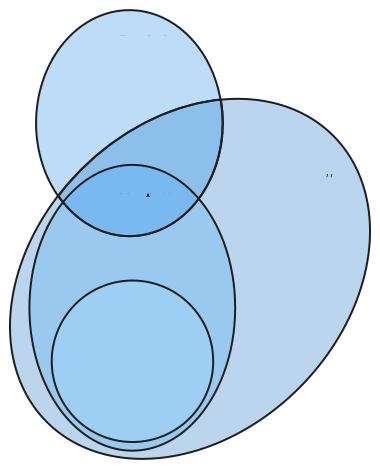
\includegraphics[width=0.5\textwidth]{figures/complexity-classes.jpg}
    \caption[Classes de complexité]{\textcolor{mydarkred}{\textit{Refaire la figure.}}}
    \label{fig:complexity-classes}
\end{figure}

L'importance des problèmes \textsf{\#P} au sein de la théorie de la complexité s'observe entre autres par le théorème de Toda~\cite{todaPPHardPolynomialTime1991}. Ce résultat marquant montre que tous les problèmes de la hiérarchie polynomiale \textsf{PH} peuvent être résolus en temps polynomial avec un oracle résolvant instantanément les problèmes \textsf{\#P}. La hiérarchie polynomiale généralise les classes de complexité \textsf{P}, \textsf{NP} et \textsf{co-NP} en capturant les classes de problèmes exprimés par une alternance de quantificateurs d'existence ($\exists$) ou d'universalité ($\forall$) (voir la définition~\ref{def:classe-np} pour un exemple contenant un seul quantificateur d'existence). Ainsi, cette hiérarchie \textsf{PH} est comprise dans la classe de complexité $\textsf{P}^{\textsf{\#P}}$, c'est-à-dire les problèmes résolubles avec un oracle \textsf{\#P}. Comme la hiérarchie polynomiale contient de nombreux problèmes importants, ce théorème suggère l'incroyable puissance des problèmes de comptage.

\begin{subtheorem}{Théorème de Toda}{toda}
    La hiérarchie polynomiale \textsf{PH} est contenue dans $\textsf{P}^{\textsf{\#P}}$.
\end{subtheorem}

\textcolor{mydarkred}{\textit{https://www.cs.cornell.edu/~sabhar/chapters/ModelCounting-SAT-Handbook-prelim.pdf}}

% L'ordinateur quantique boulverse le domaine de la complexité classique. En effet, la thèse de Church-Turing, stipulant qu'un algorithme est calculable si et seulement s'il est calculable par une machine de Turing, ne prend pas en compte les processus physiques. Le principe de Church-Turing-Deustch généralise la thèse de Church-Turing en énoncçant qu'un dispositif de calcul universel peut simuler n'importe quel processus physique. \textcolor{mydarkred}{\textit{Enlever?}}

L'ordinateur quantique bouleverse le domaine de la complexité classique. Les problèmes autrefois intraitables deviennent potentiellement résolubles efficacement à l'aide d'algorithmes quantiques. Deux nouvelles classes de complexité font alors leurs apparitions pour décrire les problèmes résolubles à l'aide de matériel informatique quantique. La classe \textsf{BQP} généralise la classe \textsf{BPP}, pour « temps polynomial probabiliste à erreur bornée », c'est-à-dire la classe de problèmes résoluble avec une probabilité d'erreur inférieure à $1/3$, pour les ordinateurs quantiques. De plus, la classe de complexité \textsf{QMA}, pour « Merlin Arthur Quantique » se définit par rapport à la classe \textsf{BQP} de manière analogue à la classe \textsf{NP} pour la classe \textsf{P}. La théorie de la complexité quantique étudie les classes de complexité quantiques dans l'objectif de déterminer les problèmes où les algorithmes quantiques comportent un avantage par rapport aux algorithmes classiques. Ce mémoire avance la recherche dans cette direction en étudiant la performance des algorithmes quantiques en comparaison avec les algorithmes classiques.

% Entre, le principe de Church-Turing-Deutsch fût proposée comme une version plus forte de la thèse de Church-Turing en utilisant les lois de la physique. 

% \textcolor{mydarkred}{\textit{Définir les problèmes de décision et de comptage ainsi que les classes de complexité de manière plus formelle (alphabet, )? Changer $B(x,y)$ par $xBy$?}}

% \textcolor{mydarkred}{\textit{Expliquer plus le théorème de Cook-Levin.}}

% \textcolor{mydarkred}{\textit{Discuter des relations entre les classes de complexité définies.}}

\textcolor{mydarkred}{\textit{Church-Turing-Deutch}}
% \textcolor{mydarkred}{\textit{Parler des problèmes d'optimisation combinatoire.}}

\textcolor{mydarkred}{\textit{Ajouter une figure sur les classes de complexité.}}
\textcolor{mydarkred}{\textit{Classe PP}}
% \textcolor{mydarkred}{\textit{Classes de complexité quantique}}

%-----------------------------------------------------------------------------%

\section{Satisfaisabilité booléenne}
\label{sec:satisfaisabilite-booleenne}
\begin{comment}
\subsection*{Plan}

\begin{enumerate}
    \item Introduire SAT
    \item Énumérer certaines applications de ce problème
    \item Faire le lien entre le problème de décision SAT et le problème de comptage SAT
    \item Introduire NAE3SAT et 1in3SAT
    \item Énoncer la réduction entre NAE3SAT/1in3SAT et 3SAT
    \item Introduire la transition de phase critique de ces problèmes
    \item Expliquer pourquoi prendre la version positive de ces problèmes n'est pas un problème
    \item Parler du comptage des problèmes SAT
    \item Introduire la transition de phase critique de ces problèmes
\end{enumerate}

\subsection*{Références}

1. Moore, Cristopher, and Stephan Mertens, The Nature of Computation (Oxford, 2011; online edn, Oxford Academic, 17 Dec. 2013), https://doi.org/10.1093/acprof:oso/9780199233212.001.0001, accessed 19 July 2024.

2. Arora, S. and Barak, B. Computational Complexity: A Modern Approach. (Cambridge University Press, Cambridge, 2009). doi:10.1017/CBO9780511804090.

3. Achlioptas, D., Chtcherba, A., Istrate, G. and Moore, C. The phase transition in 1-in-k SAT and NAE 3-SAT. Proceedings of the Annual ACM-SIAM Symposium on Discrete Algorithms (2001) doi:10.1145/365411.365760.
\end{comment}

Le problème de \textit{satisfaisabilité booléenne} ou problème SAT est particulièrement important dans la théorie de la complexité. Montré comme \textsf{NP}-complet par le théorème de Cook-Levin~\cite{cookComplexityTheoremprovingProcedures1971,levinUniversalSequentialSearch}, il fut à la base de la définition de \textsf{NP}-complétude et du problème $\textsf{P} \stackrel{?}{=} \textsf{NP}$. Celui-ci est aussi couramment utilisé dans la preuve de réductions de problèmes au sein de la classe de complexité \textsf
{NP}. Le problème SAT a une multitude d'applications, comme le diagnostic des fautes d'un circuit logique ou la planification en intelligence artificielle~\cite{marques-silvaPracticalApplicationsBoolean2008}, en partie grâce à la facilité de formuler ces applications à l'aide de formules propositionnelles.

Une \textit{formule propositionnelle}, ou une expression booléenne, est un ensemble de variables booléennes, $x_{i} \in \set{\textsc{\texttt{FAUX}}, \textsc{\texttt{VRAI}}}$, reliées par des opérateurs booléens de conjonctions (\textsc{\texttt{OU}}, $\lor$), de disjonctions (\textsc{\texttt{ET}}, $\land$) ainsi que de négation (\textsc{\texttt{NON}}, $\neg$).  Un \textit{littéral} désigne dans ce contexte une variable booléenne ou sa négation. Par exemple, l'expression $(x_{1} \land x_{2}) \lor \neg x_{3}$ est une formule booléenne composée des variables $x_{1}$, $x_{2}$ et $x_{3}$, ainsi que des littéraux $x_{1}$, $x_{2}$ et $\neg x_{3}$. Notons que l'équivalence $\textsc{\texttt{FAUX}} \leftrightarrow 0$ et $\textsc{\texttt{VRAI}} \leftrightarrow 1$ est utilisée dans ce mémoire par commodité.

Un problème SAT se décrit par une formule propositionnelle. Résoudre le problème consiste à déterminer s'il existe une combinaison de variables qui rend la formule logiquement vraie, c'est-à-dire tel que l'évaluation de celle-ci donne 1. Une telle formule est alors dite satisfaisable.

\begin{maindefinition}{Problème SAT}{probleme-sat}
    Soit une constante $n \geq 1$ et une formule propositionnelle $\varphi(x_{1}, x_{2}, \dots, x_{n})$ où $x_{i} \in \set{ 0, 1 }$.  Existe-t-il une assignation des variables $x_{1}, x_{2}, \dots, x_{n}$ telle que $\varphi$ soit satisfaisable, c'est-à-dire que $\varphi(x_{1}, x_{2}, \dots, x_{n})=1$?
\end{maindefinition}

Dans l'étude du problème SAT, les formules propositionnelles sont souvent exprimées en \textit{forme normale conjonctive} (« Conjunctive Normal Form ») (CNF). On parle alors de formules CNF. Celles-ci consistent en une conjonction d'une ou de plusieurs \textit{clauses}, où une clause est une disjonction d'un ou plusieurs littéraux. Cela implique que toute clause doit contenir au moins un littéral évaluant à 1 pour que la formule soit satisfaisable. Toute formule propositionnelle peut être réécrite en forme normale conjonctive en utilisant les lois de l'algèbre booléenne.

\begin{example}{Problème SAT}{probleme-sat}
    La formule CNF
    \begin{equation*}
        \varphi(x_{1}, x_{2}, x_{3}) = (x_{1} \lor x_{3}) \land (\neg x_{1} \lor x_{2} \lor \neg x_{3}) 
    \end{equation*}
    est satisfaisable car $\varphi(1,0,0) = (1 \lor 0) \land (\neg 1 \lor 0 \lor \neg 0) = 1$. Au contraire, la formule CNF
    \begin{equation*}
        \varphi(x_{1})= (x_{1}) \land (\neg x_{1})
    \end{equation*}
    n'est pas satisfaisable car $\varphi (x_{1}) = 0$ peu importe le choix de $x_{1}$.
\end{example}

\textcolor{mydarkred}{\textit{Tables de vérité?}}

Le problème kSAT constitue un cas spécial du problème SAT, où le nombre de littéraux appartenant à chaque clause d'une formule CNF est restreint à $k$ littéraux au maximum. Notons que le problème kSAT est trivial pour $k=1$, résoluble en temps linéaire pour $k=2$~\cite{kromDecisionProblemClass1967}, et \textsf{NP}-complet pour $k \geq 3$~\cite{karpReducibilityCombinatorialProblems1972}. Surprenamment, les problèmes de comptage correspondant, \#2SAT et \#3SAT, appartiennent tous les deux à la classe \textsf{\#P}-complet~\cite{valiantComplexityEnumerapportnReliability1979}. Ainsi, compter le nombre de solutions à un problème \textsf{NP}-complet peut être difficile même s'il est possible de trouver une solution efficacement.

Dans ce mémoire, deux variantes de 3SAT seront portées à l'étude: le problème Pas-Tous-Égaux 3SAT (« Not-All-Equal 3-Satisfiability ») (NAE3SAT) et le problème 1-dans-3 3SAT (« One-in-Three 3-Sastisfiability ») (1-in-3SAT). 
Comme le problème SAT, ces problèmes appartiennent aussi à la classe de complexité \textsf{NP}-complet. Les versions monotones de ces problèmes, où la négation de variables n'est pas permise, sont étonnament aussi \textsf{NP}-complet par le théorème de dichotomie de Schaefer~\cite{schaeferComplexitySatisfiabilityProblems1978}. Ces problèmes de décision peuvent être associés aux problèmes de comptage \#NAE3SAT et \#1-in-3SAT de la classe de complexité \textsf{\#P}.

\begin{maindefinition}{Problème NAE3SAT}{probleme-nae3sat}
    Soit une formule CNF $\varphi(x_{1}, x_{2}, \dots, x_{n})$ pour laquelle chaque clause $C$ contient au maximum 3 littéraux. Existe-t-il une assignation des variables $x_{1}, x_{2}, \dots, x_{n}$ telle que $\varphi$ soit satisfaisable tout en s'assurant que tous les littéraux de chaque clause $C$ ne soient pas égaux?
\end{maindefinition}

Notons qu'un problème NAE3SAT peut être décrit par un problème 3SAT. Soit une formule CNF $f$ exprimant un problème 3SAT. Une formule CNF $g$, représentant le problème NAE3SAT associé à $f$, est construite en transformant chaque clause $(x \lor y \lor z)$ de $f$ en $(x \lor y \lor z) \land (\neg x \lor \neg y \lor \neg z)$. Cette nouvelle contrainte renforce alors la condition supplémentaire, c'est-à-dire que les littéraux de chaque clause ne peuvent être tous égaux. Cette relation illustre bien une symétrie cachée derrière le problème NAE3SAT; chacune des variables possèdent en moyenne la même probabilité d'être vraie ou fausse.

\begin{maindefinition}{Problème 1-in-3SAT}{probleme-1in3sat}
    Soit une formule CNF $\varphi(x_{1}, x_{2}, \dots, x_{n})$ pour laquelle chaque clause $C$ contient au maximum 3 littéraux. Existe-t-il une assignation des variables $x_{1}, x_{2}, \dots, x_{n}$ telle que $\varphi$ soit satisfaisable tout en s'assurant qu'exactement un littéral de chaque clause $C$ soit logiquement vrai?
\end{maindefinition}

De la même façon que pour le problème NAE3SAT, le problème 1-in-3SAT se transforme en un problème 3SAT en transformant chaque clause $(x \lor y \lor z)$ en $(x \lor y \lor z) \land (x \lor \neg y \lor \neg z) \land (\neg x \lor y \lor \neg z) \land (\neg x \lor \neg y \lor z) \land (\neg x \lor \neg y \lor \neg z)$, de manière à encoder la contrainte additionnelle du problème 1-in-3SAT.

% \textcolor{mydarkred}{\textit{Parler du nombre de solutions.}}

%-----------------------------------------------------------------------------%

\section{Intraitabilité, approximation et optimisation}
\label{sec:intractabilite-approximation-et-optimisation}

\begin{comment}
\subsection*{Plan}

\begin{enumerate}
    \item Expliquer le concept d'intractabilité
    \item Montrer la difficulté de résoudre des problèmes computationnels de manière exacte
    \item Expliquer les advantages des méthodes approximatives (temps polynomial, applications réelles)
    \item Introduire rigoureusement le concept d'approximation
\end{enumerate}

\subsection*{Références}

Subhash Khot. Inapproximability of NP-complete Problems, Discrete Fourier Analysis, and Geometry. In Proceedings of the International Congress of Mathematicians 2010 (ICM 2010)
\end{comment}

Les problèmes algorithmiques des classes de complexité \textsf{NP}-difficile et \textsf{\#P}-difficile sont considérés comme intraitables en raison de leur complexité intrinsèque. En effet, il est improbable qu'un algorithme puisse résoudre exactement ces problèmes en temps polynomial. Par exemple, bien que certaines instances du problème SAT contenant plus d'un million de variables sont résolubles efficacement, d'autres instances de moins d'un millier de variables ne peuvent être résolus par les solveurs de pointe~\cite{froleyksSATCompetition20202021}. Cette difficulté s'accentue pour le problème \#SAT, où même une centaine de variables peut s'avérer trop complexe. 

L'intraitabilité de tels problèmes mène alors à un paradigme différent; Sachant qu'il est irréaliste de résoudre certains problèmes exactement, est-ce qu'il est possible de trouver une solution approximative de manière efficace? L'exactitude des solutions est alors sacrifié pour une performance accrue.

Les problèmes de décision ne possédant que deux solutions, oui ou non, il n'est pas possible de fournir une solution approximative. Un \textit{problème d'optimisation}, défini en conjonction à un problème de décision, est alors une notion plus adéquate pour incorporer la notion d'approximation. Ces problèmes ne cherchent plus à trouver la solution optimale, mais plutôt à obtenir une réponse suffisamment près de la valeur optimale. Un exemple de problème d'optimisation, particulièrement étudié dans le domaine de l'optimisation quantique en raison de sa simplicité d'implémentation sur du matériel informatique quantique, est le problème de coupe maximum (­« Maximum Cut ») (Max-Cut). Ce problème cherche une coupe séparant les sommets d'un graphe en deux ensembles complémentaires tel que le nombre d'arêtes séparant les deux ensemble soit maximal. Le problème Max-Cut étant \textsf{NP}-complet, il est difficile d'obtenir une coupe optimale, mais une coupe sous-optimale peut possiblement être trouvée efficacement.

Un problème d'optimisation $\Pi$ est constitué d'un ensemble d'instances valides $I_{\Pi}$, où chaque instance $x \in I_{\Pi}$ possède un ensemble de solutions faisables $S_{\Pi}(x)$. Une fonction objectif $\text{obj}_{\Pi}$, aussi nommée fonction de coût ou de perte, quantifie la qualité d'une solution approximative $y$ de $x$ en lui assignant un nombre réel. En conséquence, résoudre approximativement un problème d'optimisation correspond à minimiser ou maximiser la fonction de coût. Une mesure de succès fréquemment utilisée, autant classiquement que quantiquement, est le \textit{rapport d'approximation},
\begin{equation}
    \alpha(x, y) = \frac{\text{obj}_{\Pi}(x, y)}{\text{OBJ}_{\Pi}(x)} \,,
\end{equation}
où $\text{OBJ}_{\Pi}(x) = \min_{y} \text{obj}_{\Pi} (x, y)$. Ce type de problème est formalisé sous le nom de problème d'optimisation \textsf{NP}, mais une définition détaillée est évitée ici par simplicité. Bien que les algorithmes d'approximation heuristiques offrent fréquemment de bons résultats, ceux-ci ne possèdent aucune garantie quant à la qualité de ces solutions.

Pour pallier ce problème, des algorithmes approximatifs avec garantis sont définis en fonction de deux paramètres: la tolérance $\varepsilon$ et la confiance $\delta$. La tolérance indique l'erreur multiplicative maximale de l'approximation et la confiance indique la probabilité de succès de l'algorithme. Ce couple de paramètres est souvent utilisés pour décrire les algorithmes approximatifs.

Un \textit{algorithme d'approximation de tolérance $\varepsilon$} pallie ce problème en garantissant une solution optimale à une erreur multiplicative près~\cite{vaziraniApproximationAlgorithms2003}. Pour un problème de minimisation $\Pi$, cet algorithme produit une solution $s$ pour toutes instances $x \in I_{\Pi}$ tel que $f_{\Pi}(x, y) \leq \varepsilon(\lvert x \rvert ) \cdot \text{OBJ}(x)$ où $\lvert  x \rvert $ est la taille de l'instance et $\varepsilon \geq 1   $. Cette définition peut être détendue en permettant à l'algorithme de produire une telle solution avec une certaine probabilité. Cette variante, l'\textit{algorithme d'approximation randomisé de tolérance $\varepsilon$}, introduit des concepts pertinents pour le chapitre~\ref{cha:echantillonnage-quasi-uniforme-comptage-approximatif-randomise}.

\textcolor{mydarkred}{\textit{What is $f$?}}

\begin{subtheorem}{Algorithme d'approximation randomisé}{algorithme-approximation-randomise}
    Un algorithme d'approximation randomisé de tolérance $\varepsilon$ pour un problème de minimisation $\Pi$ est un algorithme aléatoire prenant en entrée une instance $x \in D_{\Pi}$ et une tolérance $\varepsilon$ et qui produit une solution $y \in S_{\Pi}(x)$ tel que
    \begin{equation*}
        \mathrm{ Pr } [f_{\Pi}(x, y) \leq \varepsilon(\lvert x \rvert ) \cdot \text{OBJ}(x)] \geq \frac{1}{2}
    \end{equation*}
    en temps polynomial.
\end{subtheorem}

Ces algorithmes se généralisent facilement pour un problème de maximisation.
En relaxant la condition d'exactitude, il est attendu qu'un gain en possible en terme d'efficacité. Cependant, cela n'est pas toujours aussi clair. Il existe en effet certains problèmes où trouver une solution approximative en haut d'un certain rapport d'approximation demeure intraitable tel le problème de couverture par ensembles~\cite{lundHardnessApproximatingMinimization1994}. Les algorithmes d'approximation s'appliquent aussi aux problèmes de comptage, tel que présenté à la section~\ref{sec:comptage-approximatif-randomise}.

%-----------------------------------------------------------------------------%

\section{Comptage de modèles}
\label{sec:complexite-et-bornes-sur-le-comptage}

\begin{comment}
\subsection*{Plan}

\begin{enumerate}
    \item Décrire les résultats actuels en terme de comptage exact et approximatif
    \item Énumérer les algorithmes et les solveurs modernes (DPLL, \textit{survey propagation}, \textit{belief propagation})
    \item Mentionner les meilleures bornes sur les problèmes de comptage
    \item https://arxiv.org/pdf/2002.06879
    \item Lien avec la fonction de partition
\end{enumerate}

\subsection*{Références}

1. Wahlström, M. A Tighter Bound for Counting Max-Weight Solutions to 2SAT Instances. in Parameterized and Exact Computation (eds. Grohe, M. and Niedermeier, R.) 202–213 (Springer, Berlin, Heidelberg, 2008). doi:10.1007/978-3-540-79723-419.

2. Sinclair, A. and Jerrum, M. Approximate counting, uniform generapportn and rapidly mixing Markov chains. Information and Computation 82, 93–133 (1989).
\end{comment}

% est-il possible de préciser sa complexité dans le pire des cas? Une quantité signifiante de travaux s'intéresse à cette question.

Sachant désormais que le comptage est un problème difficile, comment résoudre celui-ci? Le comptage des solutions d'une formule propositionnelle est spécifiquement connu dans la littérature sous le nom de \textit{comptage de modèles}. De nombreuses méthodes, autant exactes qu'approximatives, ont été développées pour sa résolution~\cite{biereHandbookSatisfiabilityVolume2009}. 

Les méthodes exactes attaquent généralement le problème en explorant exhaustivement l'espace des solutions possibles, de manière similaire à l'algorithme de Davis-Putnam-Logemann-Loveland (DPLL) pour les problèmes SAT~\cite{davisMachineProgramTheoremproving1962}. Les algorithmes de recherche locale pour SAT, tel l'algorithme WalkSAT, peuvent aussi être étendus pour résoudre \#SAT. Toutefois, les solveurs les plus performants actuellement sont basés sur les réseaux de tenseurs, un object mathématique provenant du domaine de la matière condensée~\cite{kourtisFastCountingTensor2019, dudekEfficientContractionLarge2020, dudekParallelWeightedModel2021}. Ces réseaux sont utiles dans de nombreux autres domaines et sont d'ailleurs utilisés dans ce travail pour la simulation de circuit quantique et font donc l'objet de l'annexe~\ref{ann:simulation-circuits-quantiques-avec-reseaux-de-tenseurs}. Bien que différents développements accentuent la taille des systèmes résolubles exactement, les solveurs ont de la difficulté à trouver l'ensemble de solutions de l'espace de recherche. 

Les méthodes approximatives allègent ce problème à l'aide d'heuristiques fournissant des estimations avec ou sans garanties. Plusieurs applications du comptage ne nécessitent pas un résultat exact; distinguer la différence entre $10^{30}$ et $10^{30}+1$ solutions n'est pas toujours pertinent. L'algorithme de Stockmeyer, qui approxime le nombre de solutions à un facteur deux avec un nombre polynomial d'appels à un oracle \textsf{NP} en s'appuyant sur les fonctions de hachage, fut un pas majeur pour le comptage approximatif~\cite{stockmeyerComplexityApproximateCounting1983}. Plusieurs modifications ont propulsé le domaine vers des performances accrues de sorte que la majorité des méthodes modernes se basent effectivement sur les fonctions de hachage. Cependant, une méthode alternative due à Jerrum, Valiant et Vazirani utilise plutôt la relation entre l'échantillonnage aléatoire de solutions et le comptage approximatif pour résoudre le problème. Malgré l'originalité de cette idée, la recherche dans cette direction s'est estompée en raison de la difficulté de l'échantillonnage de solutions avec les conditions nécessaires. Ce travail relance cette possibilité en pourvoyant une nouvelle façon d'échantillonner avec les algorithmes variationnels quantiques. Une discussion approfondie est présentée au chapitre~\ref{cha:echantillonnage-quasi-uniforme-comptage-approximatif-randomise}.

Les avancées en physique, tel les réseaux de tenseurs, présentent des avantages pour le comptage de modèle, mais l'inverse est aussi vrai. Le problème du comptage est intimement reliée au domaine de la mécanique statistique. En effet, déterminer la fonction de partition d'un système à température nulle est en réalité équivalent à un problème de comptage~\cite{timmeCountingComplexDisordered2009}. Considérons la fonction de partition $Z$ pour un Hamiltonien $H$ où l'énergie fondamentale est fixée à $E_{0} = 0$,
\begin{equation}
    Z = \sum_{i} e^{-\beta E_{i}} \,,
\end{equation}
où $\beta = \frac{1}{k_{b} T}$, $k_{B}$ est la constante de Boltzmann et $T$ est la température. Dans la limite $T \to 0$, les seuls termes non-nuls de la somme sont $e^{-\beta E_{0}}$, c'est-à-dire les termes associés aux états fondamentaux du système. Ainsi, pour un système dégénéré de $N_{0}$ états fondamentaux, la fonction de partition devient $Z = N_{0}$. Calculer la fonction de partition correspond ainsi à déterminer le nombre d'états fondamentaux.

Le développement du calcul quantique a aussi mené à de fructueux aboutissements. L'algorithme de comptage quantique prend avantage de l'algorithme de Grover et de l'algorithme d'estimation de phase quantique pour approximer le nombre de solutions à l'aide de $(\sqrt{\frac{N}{M}})$ itérations, où $M$ est le nombre de solutions, de taille exponentielle pour les problèmes SAT et $N$ est le nombre d'états possibles~\cite{brassardQuantumCounting1998}. Le nombre d'itérations nécessaires profite ainsi d'un gain quadratique par rapport à la complexité optimale classique de $O(\frac{N}{M})$.

Notons que dans tous les cas, le comptage de solutions aux formules CNF, l'objet de ce travail, ne s'effectue jamais en temps polynomial. Même les approches approximatives nécessitent un nombre exponentiel d'opérations, indiquant davantage la difficulté de ce problème.


\textcolor{mydarkred}{\textit{Model counting!}}
\textcolor{mydarkred}{\textit{Hashing based}}
\textcolor{mydarkred}{\textit{JVV}}
\textit{}
\textcolor{mydarkred}{\textit{Permanent}}

\textcolor{mydarkred}{\textit{Quantum counting?}}

\textcolor{mydarkred}{\textit{https://www.scottaaronson.com/papers/apxcount.pdf}}

\textcolor{mydarkred}{\textit{https://www.cs.cornell.edu/~sabhar/chapters/ModelCounting-SAT-Handbook-prelim.pdf}}

\textcolor{mydarkred}{\textit{https://www.cs.toronto.edu/~meel/Papers/handbook-chapter.pdf}}

\textcolor{mydarkred}{\textit{Partition function}}

%-----------------------------------------------------------------------------%

\section{Transitions de phase}
\label{sec:transitions-de-phase}

\begin{comment}
\subsection*{Plan}

\begin{enumerate}
    \item Expliquer les différentes transitions de phase et leurs intuitions
    \item Décrire l'objectif des algorithmes classiques locaux et globaux, comme le "belief propagation" ou le "survey propagation"
    \item Expliquer brièvement où se situe VQCount par rapport à ça
\end{enumerate}

\subsection*{Références}

1. Watrous, J. Quantum Computational Complexity. Preprint at https://doi.org/10.48550/arXiv.0804.3401 (2008).

2. Mézard, M. and Montanari, A. Information, Physics, and Computation. (Oxford University Press, Oxford, New York, 2009).

2. https://www.sciencedirect.com/science/article/pii/S0378437109010656

3. Survey propagation: An algorithm for satisfiability - Braunstein - 2005 - Random Structures amp; Algorithms - Wiley Online Library. https://onlinelibrary.wiley.com/doi/abs/10.1002/rsa.20057.
\end{comment}

La complexité d'une instance aléatoire d'un problème \textsf{NP} n'est pas toujours équivalente. En réalité, certaines instances sont résolubles en temps polynomial, alors que d'autres sont intraitables. Les discussions autour des classes de complexité s'intéressent principalement à la complexité dans le pire des cas pour décrire la difficulté inhérente d'un problème. Cependant, certaines instances peuvent posséder une complexité inférieure, pouvant alors être pris en avantage par certains algorithmes. 

Pour les problèmes SAT, la difficulté d'une instance aléatoire est grandement dépendante sur le rapport $\alpha = \frac{m}{n}$, où $m$ est le nombre de clauses et $n$ est le nombre de variables. Intuitivement, cette difficulté provient de l'ajout de contraintes au problème sous la forme de clauses. Plus surprenamment, la complexité d'une telle instance suit une transition de phase nommée \textit{transition de phase critique}. En effet, il existe une valeur critique $\alpha_{c}$ où les instances du problème SAT passe de satisfaisable à insatisfaisable dans la limite asymptotique de $n$. La difficulté du problème SAT est maximale juste avant cette transition. Pourquoi est-ce le cas?

Plusieurs autres transitions de phase existent avant la transition critique telle qu'illustré à la figure~\ref{fig:transitions-de-phase}. Ces transitions, similairement aux transitions de phase du modèle d'Ising, correspondent à des changements dans l'organisation de l'ensemble des solutions. Pour décrire cette réorganisation, une mesure de similarité est nécessaire pour comparer les différentes entrées au problème SAT. La \textit{distance de Hamming} entre deux chaînes de bits de même taille correspond au nombre de positions dans les chaînes où les bits correspondants diffèrent. 


Avant la première transition de phase, la \textit{transition de phase de regroupement}, toutes les solutions d'une instance du problème SAT sont situées au sein du même amas, chacune à une distance d'Hamming polynomiale selon la taille de l'instance.

\textit{transition de phase de congélation}



\begin{figure}[h]
    \centering
    \includegraphics[width=1\textwidth]{figures/phase-transitions.pdf}
    \caption[Transitions de phase du problème SAT]{Schéma des transitions de phase du problème SAT selon le rapport du nombre de clauses au nombre de variables $\alpha$. Les transitions de phases illustrées sont la transition de regroupement $\alpha_{\text{clust}}$, la transition de condensation $\alpha_{\text{cond}}$, la transition de congélation $\alpha_{\text{rigid}}$ et la transition de satisfaisabilité $\alpha_{c}$.}
    \label{fig:transitions-de-phase}
\end{figure}

Les approches locales semblent échouer à la transition de condensation, alors que la difficulté du problème SAT semble provenir de la transition de congélation.


NAE3SAT: $\alpha_{c} \approx 2.1$~\cite{achlioptasPhaseTransition1ink2001}
1-in-3SAT: $\alpha_{c} \approx 2/3$~\cite{raymondPhaseDiagram1in32007}

\textcolor{mydarkred}{\textit{Pourquoi transition dynamique?}}

\textcolor{mydarkred}{\textit{Parler du nombre de solutions.}}

\textcolor{mydarkred}{\textit{Locked problems.}}

Les instances du problème \#1-in-3SAT près du seuil critique appartiennent à la catégorie des problèmes bloqués. Les problèmes \#P dans ce régime sont parmi les plus difficiles~\cite{zdeborovaStatisticalPhysicsHard2008}.

\textcolor{mydarkred}{\textit{Voir papier de stefanos fast counting, plus d'informations et de références.}}

\textcolor{mydarkred}{\textit{Algorithme local vs global}}

\chapter{Échantillonnage quasi uniforme et comptage approximatif randomisé}
\label{cha:echantillonnage-quasi-uniforme-comptage-approximatif-randomise}

Les problèmes de décision, ou d'existence, et de comptage tels qu'introduits dans le chapitre précédent ne forment qu'une infime partie des problèmes étudiés dans la théorie de la complexité. Ces problèmes se cadrent notamment parmi les problèmes suivants:

\begin{enumerate}[(1)]
    \item \textbf{Existence}: Existe-t-il une solution au problème?
    \item \textbf{Construction}: Construire une solution au problème.
    \item \textbf{Génération uniforme}: Générer uniformément et aléatoirement une solution au problème.
    \item \textbf{Comptage} Combien de solutions satisfont le problème?
\end{enumerate}

Il n'est pas évident de prime abord de comparer la complexité de ces problèmes. Toutefois, dans une publication marquante pour le domaine de la complexité du comptage, Jerrum, Valiant et Vazirani offrent une unique perspective sur l'écart de complexité entre ces différents problèmes~\cite{jerrumRandomGenerationCombinatorial1986}. Les auteurs suggèrent d'abord que la génération uniforme est strictement plus difficile que la construction, et donc que l'existence, car la construction est évidemment au moins aussi difficile que l'existence. De plus, ils avancent que la génération uniforme est plus simple que le comptage, tout en offrant une réduction de la génération uniforme au comptage approximatif. En relaxant le comptage approximatif au comptage approximatif randomisé, ils établissent une correspondance entre ce dernier et la génération quasi uniforme.

Ce travail éclaircit la compréhension de la théorie de la complexité, particulièrement pour la génération uniforme et du comptage. La dernière correspondance entre le comptage approximatif randomisé et la génération quasi uniforme s'avère particulièrement intéressante et forme la base du travail de ce mémoire. Cette interréduction mène en effet à un algorithme de comptage approximatif résolvant approximativement certains problèmes de comptage, possédant la propriété d'auto-réductibilité, à l'aide d'un générateur de solutions quasi uniforme. Par souci de commodité, cet algorithme est appelé l'\textit{algorithme de JVV} selon le nom de ses auteurs. Parmi ses principaux attraits est sa capacité à obtenir un compte approximatif avec un nombre polynomial d'appels au générateur de solutions, sous la condition que ce dernier soit génère une distribution de solutions suffisamment uniforme. Cette propriété s'avère particulièrement utile pour les problèmes possédant un nombre exponentiel de solutions, comme le problème SAT.

Les trois concepts nécessaires à l'algorithme de JVV sont formalisés dans cette section: l'auto-réductibilité à la section~\ref{sec:auto-reductibilite}, l'échantillonnage quasi uniforme à la section~\ref{sec:echantillonnage-quasi-uniforme} et le comptage approximatif randomisé à la section~\ref{sec:comptage-approximatif-randomise}. Pour conclure, la section~\ref{sec:algorithme-jvv} présente une description en profondeur de l'algorithme de JVV.

%-----------------------------------------------------------------------------%

\section{Auto-réductibilité}
\label{sec:auto-reductibilite}

Avant d'introduire le concept d'auto-réductibilité, il est utile de définir une notion supplémentaire. Les problèmes abordés dans l'introduction de ce chapitre concernent généralement des objets mathématiques discrets, tels que les formules propositionnelles, les graphes, les permutations, et bien plus. Ces objets se regroupent sous une même ombrelle, nommée \textit{structure combinatoire}, définie comme un système discret fini comportant des éléments et des relations bien définies. Par exemple, une formule propositionnelle, composée de variables booléennes et de contraintes sous forme d'opérateurs booléens, est associée à un ensemble discret de solutions. Conséquemment, le domaine de l'\textit{énumération combinatoire} cherche à déterminer le nombre d'éléments satisfaisant la relation. Pour le problème SAT, cela consiste à trouver le nombre d'assignations satisfaisant la formule propositionnelle. De manière similaire, l'\textit{optimisation combinatoire} tente de trouver la meilleure solution possible au problème.

L'\textit{auto-réductibilité} (« self-reducibility ») est un concept complexe, essentiel à la compréhension du calcul et de la complexité, découlant de l'introduction de la \textit{réduction automatique} (« autoreducibility »)~\cite{trakhtenbrotAutoreducibility1970, selkeAutoreducibilityFriendsMeasuring2006}. Ces concepts sont particulièrement importants dans le contexte de génération aléatoire et du comptage approximatif, mais aussi pour la réduction entre le problème de décision et les problèmes de recherche.

\begin{subdefinition}{Réduction automatique}{auto-reductibilite}
    Un problème algorithmique est dit \textit{automatiquement réductible} s'il peut être résolu par un algorithme résolvant d'autres instances du même problème, sans que l'algorithme puisse interroger l'instance particulière qu'il cherche à résoudre.
\end{subdefinition}

Les problèmes automatiquement réductibles contiennent de l'information d'appartenance redondante, c'est-à-dire qu'il existe une structure dans l'ensemble de problèmes pouvant être exploitée pour simplifier le calcul d'une instance donnée. Ainsi, un algorithme peut résoudre une instance en utilisant l'information redondante présente dans d'autres instances, évitant ainsi les requêtes directes à l'instance en question. Connaître la solution à un autre problème peut alors simplifier la résolution du problème initial. 

Par exemple, imaginons un casse-tête composé de nombreuses pièces, chacune s'emboitant d'une manière spécifique avec certaines autres. Est-il possible d'assembler toutes les pièces pour former une image complète? Bien entendu, en observant seulement chaque pièce individuellement, répondre à cette question est plutôt ardu. Une stratégie alternative, plus intuitive, consiste à construire le casse-tête progressivement. On choisit d'abord une seule pièce, et puis on tente d'ajouter les autres une à une, en posant à chaque fois la question suivante: est-il possible d'emboîter correctement cet ensemble de pièces? Cette question, qui représente une instance différente du même problème, s'avère bien plus simple! Si aucun ajout ne fonctionne, alors le casse-tête est impossible à assembler. Si au moins une des autres pièces s'emboîte correctement, alors les deux pièces sont emboîtées et la procédure est répétée avec ce nouveau sous-ensemble. Si toutes les pièces peuvent être successivement ajoutées et assemblées correctement, alors le casse-tête est résoluble. La question initiale a ainsi été répondue en interrogeant uniquement des instances différentes, ici partielles, du problème, sans résoudre directement le casse-tête. Notons que cet exemple ne donne qu'un exemple intuitif de la réduction automatique sans y correspondre strictement parlant. En effet, la méthode employée est exploratoire et n'exploite pas explicitement la structure du problème. Un exemple plus formel, le problème SAT, est décrit plus bas.

Pour discuter de la génération aléatoire et le comptage approximatif, l'\textit{auto-réductibilité descendante}, une forme limitée de la réduction automatique, est une définition plus adéquate. En effet, cette condition est nécessaire à l'application de l'algorithme JVV.

\begin{maindefinition}{Auto-réductibilité descendante}{auto-reductibilite-informel}
    Un problème algorithmique est dit \textit{auto-réductible descendant} si les instances de ce problème peuvent être résolues à partir d'instances de taille strictement inférieure.
\end{maindefinition}

Cette propriété s'éclaircit en prenant le problème SAT comme exemple. L'auto-réductibilité appliquée au problème de satisfaisabilité s'exprime facilement avec la relation suivante~\cite{hemaspaandraPowerSelfReducibilitySelectivity2020}:

\begin{relation}{Auto-réductibilité pour les problèmes SAT}{auto-reductibilite-sat}
    Soit une constante $n \geq 1$ et un problème SAT décrit par la formule propositionnelle $\varphi(x_{1}, x_{2}, \dots, x_{n})$ où $x_{i} \in \set{ 0, 1 }$. Alors,
    \begin{equation*}
        \varphi(x_{1}, x_{2}, \dots, x_{n}) = 1 \iff \varphi(x_{1}=0, x_{2}, \dots, x_{n}) = 1 \lor \varphi(x_{1}=1, x_{2}, \dots, x_{n}) = 1
    \end{equation*}
\end{relation}

Cette relation implique que l'ensemble de solutions d'une instance donnée peut être exprimé comme l'ensemble de solutions de deux instances plus petites du problème. Supposons que l'on souhaite résoudre une instance du problème SAT décrit par la formule CNF $\varphi(x_{1}, x_{2}, \dots, x_{n})$. Soit $\varphi_{0} = \varphi(x_{1}=0, \dots, x_{n})$ et $\varphi_{1} = \varphi(x_{1}=1, \dots, x_{n})$ deux sous-instances de l'instance $\varphi$, où la variable $x_{1}$ est remplacée par 0 et 1 respectivement. Ce faisant, la formule $\varphi$ est alors raccourcie, comme certaines clauses sont satisfaites ou du moins réduites. Pour que l'instance $\varphi$ soit satisfaisable, il est nécessaire qu'au moins une des sous-instances $\varphi_{0}$ et $\varphi_{1}$ soit satisfaisable. Dans le cas contraire, l'instance originale $\varphi$ ne peut être satisfaisable, car il n'existe pas de solutions peu importe la valeur de $x_{1}$. Ainsi, il suffit de considérer la disjonction des sous-problèmes possibles du problème original pour résoudre ce dernier. Les sous-problèmes obtenus étant aussi des formules propositionnelles, ceux-ci peuvent aussi être décomposés en problème de taille inférieure récursivement. 

Notons qu'il n'est pas nécessaire de construire la relation~\ref{rel:auto-reductibilite-sat} avec la variable $x_{1}$, n'importe quelle variable $x_{i}$ peut aussi être utilisée. Notons aussi que le problème SAT est décrit comme une auto-réductibilité à longueur décroissante 2-disjonctive. Ici, 2-disjonctive fait référence à une formule propositionnelle composée d'une disjonction de conjonctions de deux variables au plus. Une longueur décroissante ou descendante signifie que l'algorithme résout des instances de taille strictement inférieure.

La relation~\ref{rel:auto-reductibilite-sat} exemplifie une deuxième façon de voir l'auto-réductibilité: la résolution partielle d'une instance d'un problème laisse une plus petite instance du même type de problème. Une interprétation alternative est qu'une instance peut être résolue en résolvant des plus petites instances et en assemblant les sous-instances ensemble, tel l'assemblage d'un casse-tête. 

Afin d'obtenir une meilleure perspective sur la notion d'auto-réductibilité, il est pertinent d'exprimer la structure d'une relation auto-réductible $\varphi$ sous la forme d'un arbre orienté, nommé \textit{arbre d'auto-réductibilité}, illustré à la figure~\ref{fig:arbre-auto-reductibilite}. Dans cet arbre, les sommets représentent à la fois une chaîne de bits $w$ de taille $m$ et une instance de problème $\varphi_{w}$, où $\varphi_{w}$ représente la sous-instance du problème $\varphi$ dont les premières variables sont remplacées par la chaîne de bits $w$. Le sous-problème est alors dit \textit{fixé} par le préfixe $w$. Les arêtes du graphe représentent l'assignation d'une variable. La racine de l'arbre correspond à l'instance du problème initial $\varphi$ ainsi qu'à une solution partielle nulle. Les enfants de cette racine sont par la suite donnés par les sous-instances $\varphi_{w}$ pour tous les préfixes $w$ de taille $1$ possibles. Le reste de l'arbre est défini récursivement de la même manière en augmentant la taille $m$ de la chaîne de bits $w$ à chaque niveau jusqu'aux feuilles de l'arbre. Ces feuilles représentent finalement une entrée au problème $\varphi$, étant soit une solution ou une non-solution au problème.

\begin{figure}[h]
    \centering
    \includegraphics[width=0.6\textwidth]{figures/self-reducibility-tree.pdf}
    \caption[Arbre d'auto-réductibilité]{Un exemple de l'arbre d'auto-réductibilité pour une formule CNF $\varphi(x_{1}, x_{2})$. Les sommets représentent des attributions de littéraux dans $\varphi$ alors que les arêtes orientées indiquent l'affectation d'un littéral.}
    \label{fig:arbre-auto-reductibilite}
\end{figure}

L'auto-réductibilité est simplement généralisable aux problèmes dont les variables peuvent prendre $d$ valeurs, dit auto-réductibilité $d$-disjonctive, en prenant la disjonction sur les $d$ valeurs possibles. Le degré de l'arbre est en conséquence donné par $d$. Notons aussi que l'arbre d'auto-réductibilité est parfois défini tel que les feuilles correspondent uniquement à des solutions au problème auto-réductible. Dans ce cas, les non-solutions ne sont pas incluses dans les ramifications de l'arbre.

Par complétude, une définition rigoureuse de l'auto-réductibilité dans le sens de Schnorr~\cite{schnorrOptimalAlgorithmsSelfReducible1976} est donnée en suivant les explications de Jerrum, Valiant et Vazirani~\cite{jerrumRandomGenerationCombinatorial1986}. Celle-ci permet l'introduction d'un langage pertinent pour le reste de ce chapitre.

\begin{maindefinition}{Auto-réductibilité descendante}{auto-reductibilite-formel}
    Soit $\Sigma^{*}$ un ensemble fixe et fini encodant les instances d'un problème ainsi que leurs solutions. Soit $R \subseteq \Sigma^{*} \times \Sigma^{*}$ une relation binaire assignant à chaque instance de problème $x \in \Sigma^{*}$ un ensemble de solutions $\set{ y \in \Sigma^{*} : xRy }$. Une relation $R \subseteq \Sigma^{*} \times \Sigma^{*}$ est auto-réductible si et seulement si
    \begin{enumerate}[(1)]
        \item il existe une fonction calculable en temps polynomial $g \in \Sigma^{*} \to \mathbb{N}$ tel que $xRy \implies \lvert y \rvert = g(x)$;
        \item il existe une fonction calculable en temps polynomial $\psi \in \Sigma^{*} \times \Sigma^{*} \to \Sigma^{*}$ et $\sigma \in \Sigma^{*} \to \mathbb{N}$ satisfaisant
        \begin{align*}
            & \sigma(x)=O(\log |x|) \,, \\
            & g(x)>0 \Rightarrow \sigma(x)>0 \quad \forall x \in \Sigma^{\star} \,, \\
            & |\psi(x, w)| \leqslant|x| \quad \forall x, w \in \Sigma^{\star} \,,
        \end{align*}
        et tel que, pour tout $x \in \Sigma^{*}$ et $y=y_1 \ldots y_n \in \Sigma^{*}$, 
        \begin{equation*}
            \left ( x, y_1 \ldots y_n \right ) \in R \Leftrightarrow \left ( \psi \left( x, y_1 \ldots, y_{\sigma(x)} \right), y_{\sigma(x)+1} \ldots y_n \right ) \in R \,.
        \end{equation*}
    \end{enumerate}
\end{maindefinition}

Démystifions cette définition. L'ensemble $\Sigma$ est un alphabet fini encodant à la fois les instances du problème et ses solutions. Le problème SAT est un exemple de relation binaire $R$, où $x$ encode une formule booléenne et $y$ encode une assignation satisfaisable parmi l'ensemble des entrées possibles $\Sigma^{*}$ tel que
\begin{equation}
    \begin{aligned}
    R = \{ (x,y) : \ & x \in \Sigma^{*} \text{ encode une formule booléenne } B, \\ 
    & y \in \Sigma^{*} \text{ est une assignation satifaisable de } B \} \,.
    \end{aligned}
\end{equation}
La notation $xRy$ signifie que $y$ est une solution valide à l'instance $x$. La première condition implique que la taille des solutions, donnée par la fonction $g$, est calculable en temps polynomial. La deuxième condition implique que, pour une instance $x$ et un préfixe $w$ de taille $\sigma(x)$ de n'importe quelle solution $y$ au problème $x$, la fonction $\psi$ donne une instance $x'$ dont les solutions sont exactement celles qui, lorsque concaténées avec $w$, forment les solutions de $x$. La fonction $\sigma$ donne alors la granularité des solutions, c'est-à-dire le nombre de caractères de $y$ utilisés pour réduire l'instance $x$. Plus précisément, $\psi(x, w) \leq \lvert x \rvert$ assure que la taille du problème diminue à mesure que la réduction se poursuit. L'implication $g(x) > 0 \implies  \sigma(x) > 0$ signifie que la réduction continue tant que la taille de l'instance $x$ est non nulle. La dernière relation énonce que la résolution du problème pour $\braket{x, y}$ peut être réduite à la résolution d'instances de taille inférieure, c'est-à-dire que $(x, y_{1}\dots y_{n})$ est reliée à $(\psi(x, y_{1}\dots y_{\sigma (x)}), y_{\sigma(x)+1}\dots y_{n})$.

Tous les problèmes \textsf{NP}-complet sont auto-réductibles~\cite{goldreichComputationalComplexityConceptual2008}, mais ce n'est pas le cas pour tous les problèmes de la classe \textsf{NP}~\cite{khullerPlanarGraphColoring1991a}. De nombreux problèmes \textsf{NP} sont aussi auto-réductible descendant. Ces observations impliquent que l'algorithme de JVV s'applique en théorie à de nombreux problèmes intéressants. Toutefois, trouver une relation auto-réductible en pratique n'est pas toujours évident.

La définition de l'auto-réductibilité utilisée dans cette section s'applique principalement à l'équivalence entre l'échantillonnage quasi uniforme et le comptage approximatif randomisé. Cependant, une définition alternative~\cite{goldreichComputationalComplexityConceptual2008} est souvent introduite pour l'équivalence entre les problèmes de décision et les problèmes de recherche, où un problème de recherche ne demande pas seulement de montrer l'existence d'une solution, mais de construire une telle solution. Si un problème est auto-réductible à ce sens, alors le problème de recherche est de la même complexité que le problème de décision. 

%-----------------------------------------------------------------------------%

\section{Échantillonnage quasi uniforme}
\label{sec:echantillonnage-quasi-uniforme}

L'\textit{échantillonnage uniforme} de structures combinatoires consiste à générer aléatoirement des solutions de manière uniforme, c'est-à-dire avec une probabilité suivant la distribution de probabilité uniforme des solutions, à un problème donné. Le problème de génération uniforme est assez méconnu, mais possède plusieurs applications, dont la construction d'éléments représentatifs d'un ensemble, la formulation de conjectures pour un ensemble ou la vérification fonctionnelle du matériel informatique~\cite{jerrumFastUniformGeneration1990, chakrabortyScalableNearlyUniform2013}.

La génération uniforme étant une demande plutôt rigide, il est parfois nécessaire de relaxer la condition d'uniformité pour une quasi-uniformité. Une distribution quasi uniforme est en pratique indiscernable d'une distribution uniforme, mais ce relâchement facilite certaines preuves. La \textit{distance en variation totale} est une mesure de distance statistique définie entre deux distributions de probabilité, déterminant la similitude entre ces distributions. Cette mesure permet, entre autres, de déterminer dans quelle mesure une distribution quasi uniforme se rapproche de la distribution uniforme.

\begin{subdefinition}{Distance en variation totale}{tvd}
    Soit deux distributions de probabilité $P$ et $Q$ définies sur un ensemble dénombrable $\chi$. La distance en variation totale est
    \begin{equation*}
        \lVert P - Q \rVert_{TV} \equiv \frac{1}{2} \sum_{x \in \chi} \lvert P(x) - Q(x) \rvert \,. 
    \end{equation*}
\end{subdefinition}

Une distribution est alors dite quasi uniforme si sa distance en variation totale avec la distribution uniforme est suffisamment petite. Une définition commune demande que cette distance diminue proportionnellement avec l'inverse de la taille du problème. Un \textit{échantillonneur quasi uniforme de tolérance $\xi$} génère alors des solutions selon une distribution de probabilités où la distance en variation totale entre celle-ci et la distribution uniforme est plus petite que $\xi$~\cite{jerrumCountingSamplingIntegrating2003}.

\begin{maindefinition}{Échantillonneur quasi uniforme}{fpaus}
    Un échantillonneur quasi uniforme pour une relation binaire $R \subseteq \Sigma^{*} \times \Sigma^{*}$ assignant à chaque instance d'un problème $x \in \Sigma^{*}$ un ensemble de solutions $S(x) = \set{ y \in \Sigma^{*} : xRy }$, est un algorithme aléatoire prenant en entrée une instance $x$ et une tolérance d'échantillonnage $\xi > 0$ et générant une solution $y \in S(x)$ tel que
    \begin{equation*}
        \lVert Y - U \rVert_{TV} \leq \xi \,,
    \end{equation*}
    où $Y$ est la distribution de probabilité de $y$ et $U$ est la distribution de probabilité uniforme sur $S(x)$. Si l'algorithme s'exécute en temps borné par une fonction polynomiale en $\lvert x \rvert$ et en $\ln (\xi^{-1})$, on parle d'échantillonneur quasi uniforme pleinement polynomial (« Fully Polynomial Almost Uniform Sampler») (FPAUS).
\end{maindefinition}

Une notion supplémentaire est introduite dans ce mémoire afin de simplifier la notation. La \textit{non-uniformité}, de manière similaire à la distance en variation totale, décrit la distance entre une distribution de probabilité $P$ et la distribution de probabilité uniforme $U$. Un échantillonneur quasi uniforme de tolérance $\xi$ possède en conséquence une non-uniformité plus petite que $\xi$.

\begin{maindefinition}{Non-uniformité}{non-uniformite}
    Soit la distribution de probabilité $P$ et la distribution de probabilité uniforme $U$ telles que $U(x) = 1/\lvert x \rvert$ définies sur un ensemble dénombrable $\chi$. La non-uniformité est
    \begin{equation*}
        \eta \equiv \frac{1}{2} \sum_{x \in \chi} \lvert P(x) - U(x) \rvert \,. 
    \end{equation*}
\end{maindefinition}

%-----------------------------------------------------------------------------%

\section{Comptage approximatif randomisé}
\label{sec:comptage-approximatif-randomise}

Comme mentionné au chapitre~\ref{cha:complexite-du-denombrement}, les problèmes de comptage sont d'une grande complexité et nécessitent en pratique des méthodes approximatives pour la résolution de problèmes de grandes tailles. Le \textit{comptage approximatif randomisé} simplifie davantage les attentes en ne demandant une solution approximative valide qu'avec une certaine probabilité. Un \textit{schéma d'approximation randomisé de tolérance $\varepsilon$} se définit de manière similaire à l'algorithme d'approximation pour l'optimisation, décrit à la section~\ref{sec:intractabilite-approximation-et-optimisation}~\cite{jerrumCountingSamplingIntegrating2003}. 

\begin{maindefinition}{Schéma d'approximation randomisé}{fpras}
    Un schéma d'approximation randomisé pour un problème de comptage $f: \Sigma^{*} \to \mathbb{N}$ est un algorithme randomisé prenant en entrée une instance d'un problème $x \in \Sigma^{*}$ et une tolérance d'erreur $\varepsilon > 0$ et qui génère un nombre rationnel $N \in \mathbb{Q}$ tel que, pour toute instance $x$,
    \begin{equation*}
        \mathrm{ Pr }\left[(1+\varepsilon)^{-1} f(x) \leq N \leq (1+\varepsilon)f(x)\right] \geq \frac{3}{4} .
    \end{equation*}
    Si l'algorithme s'exécute en temps borné par une fonction polynomiale en $\lvert x \rvert$ et $\varepsilon^{-1}$, alors on parle de schéma d'approximation randomisé pleinement polynomial (« Fully Polynomial Randomized Approximation Scheme ») (FPRAS).
\end{maindefinition}

Dans la définition précédente, un problème de comptage $f: \Sigma^{*} \to \mathbb{N}$ associe une instance d'un problème $x \in \Sigma^{*}$ avec son nombre de solutions $f(x)$. Le schéma d'approximation randomisé estime alors $f(x)$ par un nombre rationnel $N \in \mathbb{Q}$. La valeur $3/4$ est un nombre arbitraire pouvant être remplacé par n'importe quel nombre dans l'intervalle ouvert $(1/2, 1)$. Ce nombre, représentant la confiance de succès du schéma, peut être augmenté à n'importe quelle valeur $1-\delta$ pour $\delta > 0$ au coût d'un facteur multiplicatif $O(\log(\delta^{-1}))$. Pour ce faire, il suffit de répéter le schéma original $O(\log(\delta^{-1}))$ fois et de prendre la médiane des résultats obtenus.   

%-----------------------------------------------------------------------------%

\section{Algorithme de Jerrum-Valiant-Vazirani}
\label{sec:algorithme-jvv}

Le travail de Jerrum, Valiant et Vazirani~\cite{jerrumRandomGenerationCombinatorial1986} (voir aussi~\cite{broderHowHardIt1986, sinclairAlgorithmsRandomGeneration1993}) établit une correspondance entre l'échantillonnage quasi uniforme et le comptage approximatif randomisé. Pour montrer celle-ci, les auteurs présentent deux algorithmes permettant le passage d'un problème à l'autre. Bien que la réduction du comptage à l'échantillonnage est intéressante, elle ne sera discutée que brièvement à la fin de la section comme la réduction d'importance est ici son inverse. L'algorithme de comptage approximatif randomisé, surnommé \textit{algorithme de JVV}, permet de trouver le nombre de solutions d'un problème auto-réductible de la classe \textsf{\#P} à une erreur multiplicative près avec un nombre polynomial d'appels à un générateur de solution quasi uniforme. Le comptage approximatif randomisé est utilisé plutôt que le comptage approximatif en raison de l'impossibilité d'obtenir un résultat déterministe à partir d'une procédure aléatoire.

\begin{maintheorem}{Algorithme de JVV}{algorithme-jvv}
    Si un problème auto-réductible dans \textsf{\#P} de taille $n$ admet un générateur de solutions avec une non-uniformité $\eta = O(1 / n)$, alors le nombre de solutions peut être approximé à une erreur multiplicative $O(\eta n)$ avec une haute probabilité en utilisant un nombre polynomial d'appels au générateur.
\end{maintheorem}

En exigeant un échantillonneur quasi uniforme pleinement polynomial (FPAUS), l'algorithme de JVV fournit un schéma d'approximation randomisé pleinement polynomial (FPRAS) pour le comptage approximatif de relations auto-réductibles. Plus précisément, pour un problème de $n$ variables, $O(\frac{n^{2} \log \delta^{-1}}{\varepsilon^{2}})$ échantillons sont nécessaires pour obtenir un compte approximatif de tolérance $\varepsilon$ et de confiance $\delta$.

Comment est-ce que l'algorithme de JVV opère? Commençons par introduire l'idée principale derrière l'algorithme pour ensuite donner un exemple simple et compléter avec une description plus formelle. 

Pour mieux comprendre son exécution, l'arbre d'auto-réductibilité, présenté à la section~\ref{sec:auto-reductibilite}, est employé. L'algorithme de JVV implique de se déplacer vers le haut ou vers le bas de cet arbre, en s'intéressant à toutes les sous-instances en chemin. Supposons qu'il soit possible d'échantillonner uniformément les solutions de n'importe quelle instance de taille $n$ du problème SAT (la généralisation à un échantillonneur quasi uniforme est effectuée plus bas). Commençons par échantillonner des solutions au problème initial $\varphi$ représenté par la racine de l'arbre. Soit $P_{0}$ et $P_{1}$ les probabilités que la première variable $x_{1}$ prenne respectivement les valeurs $0$ et $1$, calculées à partir des solutions échantillonnées. Ces probabilités reflètent la proportion de solutions dans chaque sous-arbre. Notons la valeur la plus probable par $w_{1}$. Descendons l'arbre vers l'enfant le plus probable $\varphi_{w_{1}}$, représentant la formule $\varphi$ réduite par le préfixe $w_{1}$, en gardant en mémoire la probabilité $P_{w_{1}}$. Comme l'échantillonneur peut aussi résoudre le problème subséquent, nous pouvons encore déterminer la valeur la plus probable $w_{2}$ de la variable suivante $x_{2}$ à partir de la probabilité $P_{w_{1}w_{2}}$. Le processus est répété jusqu'à atteindre les feuilles de l'arbre, en sauvegardant les probabilités $P_{w_{1} w_{2} \dots w_{i}}$ le long du chemin $w_{1} w_{2} \dots w_{i}$ choisi. Au dernier noeud avant les feuilles, nous obtenons une solution donnée par $w_{1} w_{2} \dots w_{n}$ avec une probabilité $P_{w_{1} w_{2} \dots w_{n}}$. Comme nous sommes à la base de l'arbre, cette probabilité indique le nombre de solutions que possède la dernière sous-instance. En effet, ce sous-arbre contient nécessairement $\frac{1}{P_{w_{1} w_{2} \dots w_{n}}}$ solutions, car il y a nécessairement une ou deux solutions à la dernière sous-instance. En remontant l'arbre, on remarque que la sous-instance précédente contient $\frac{1}{P_{w_{1} w_{2} \dots w_{n-1}}}$ fois plus de solutions. Par conséquent, le nombre de solutions dans cette partie de l'arbre est de $\frac{1}{P_{w_{1} w_{2} \dots w_{n}}} \cdot \frac{1}{P_{w_{1} w_{2} \dots w_{n-1}}}$. Continuant cette procédure jusqu'à la racine, nous trouvons que le nombre de solutions au problème $\varphi$ est donné par 
\begin{equation}
    \label{eq:jvv-probabilities}
    N = \frac{1}{P_{w_{1}}} \cdot \frac{1}{P_{w_{1} w_{2}}} \dots \frac{1}{P_{w_{1} w_{2} \dots w_{n}}} = \frac{N}{N_{w_{1}}} \cdot \frac{N_{w_{1}}}{N_{w_{1} w_{2}}} \dots \frac{N_{w_{1} w_{2} \dots w_{n-1}}}{N_{w_{1} w_{2} \dots w_{n}}} \,,
\end{equation}
où $N_{w_{1} \dots w_{i}}$ est le nombre de solutions au problème $\varphi_{w_{1}, \dots, w_{i}}$. En exprimant les probabilités sous la forme de rapport entre le nombre de solutions d'un plus petit sous-arbre au sein d'un sous-arbre, comme montré à l'équation~\ref{eq:jvv-probabilities}, nous remarquons que tous les termes s'annulent à l'exception de $N$ et de $N_{w_{1}w_{2}\dots w_{n}}$. Ce dernier étant nécessairement $1$, la multiplication de l'inverse des probabilités donne bien le nombre de solutions au problème.

Éclaircissons maintenant cette idée à l'aide d'un exemple simple illustré à la figure~\ref{fig:algorithme-jvv}. Considérons une instance du problème SAT décrite par la formule CNF $\varphi(x_{1}, x_{2}) = \neg x_{1} \lor x_{2}$, dont les solutions sont les couples $(0,0)$, $(0,1)$ et $(1,1)$. Un arbre est construit de manière à représenter toutes les sous-instances de l'instance originale. La racine de l'arbre représente le problème initial $\varphi$ et ses deux variables $x_{1}$ et $x_{2}$. La première couche représente les sous-problèmes $\varphi_{0}$ et $\varphi_{1}$ où la première variable du problème $\varphi$ est remplacée par 0 et 1 respectivement. Les feuilles représentent les assignations possibles au problème $\varphi$, c'est-à-dire $00$, $01$, $10$ et $11$, comme toutes les variables sont fixées à une certaine valeur. Les arêtes de l'arbre décrivent la probabilité de l'assignation des variables. Par exemple, la probabilité $P_{11}=1$ indique que les échantillons générés à partir du sous-problème $\varphi_{1}$ commencent par le préfixe $11$ avec une probabilité $1$. Maintenant que l'arbre d'auto-réductibilité est construit, comptons le nombre de solutions à la formule $\varphi(x_{1}, x_{2})$. En échantillonnant l'instance originale, nous trouvons que les échantillons possèdent une probabilité $P_{0}=2/3$ de commencer avec la variable $x_{1} = 0$. La sous-instance $\varphi_{0} = \varphi(0, x_{1})$ est donc choisie, comme il s'agit de l'enfant le plus probable, et de nouvelles solutions sont générées. Nous remarquons que celles-ci possèdent la même probabilité $P_{00} = P_{01} =\frac{1}{2}$ de commencer par le préfixe $00$ que par le préfixe $01$. Après avoir choisi le préfixe $01$, le compte est obtenu avec $N = (P_{0} \cdot P_{01})^{-1} = (\frac{2}{3} \cdot \frac{1}{2})^{-1} = 3$.

\begin{figure}[h]
    \centering
    \includegraphics[width=0.6\textwidth]{figures/jvv-algorithm.pdf}
    \caption[Algorithme de Jerrum-Valiant-Vazirani]{Un exemple de l'arbre d'auto-réductibilité dans l'algorithme JVV pour une formule CNF $\varphi(x_{1}, x_{2})$. Les sommets représentent des attributions de littéraux dans $\varphi$, avec les solutions représentées par des carrés bleus et les non-solutions par des losanges rouges. Les arêtes orientées indiquent l'affectation d'un littéral ainsi que sa probabilité associée. En suivant le chemin des probabilités maximales, illustré par une ligne pleine, le compte est obtenu avec $N = (P_{0} \cdot P_{01})^{-1} = 3$.}
    \label{fig:algorithme-jvv}
\end{figure}

Quelques notes sont ici nécessaires. Le chemin des probabilités maximales est choisi, car une meilleure précision est atteinte avec un plus grand nombre de différentes solutions échantillonnées. De plus, ce choix évite d'obtenir une probabilité nulle, ce qui arrive si le sous-arbre ne possède aucune solution. Jusqu'à maintenant, le générateur a été considéré comme uniforme. Il est cependant possible d'utiliser une distribution quasi uniforme, qui introduit une petite erreur additionnelle pouvant être absorbée dans la tolérance $\varepsilon$.

Maintenant que l'intuition derrière l'algorithme de JVV est éclaircie, décrivons plus formellement celui-ci. Supposons que le nombre exact de solutions pour une instance de taille $n$ du problème SAT est de $N$. Notons $x_{:m}$ le préfixe de taille $m$ de la chaîne de bits $x$ et $N_{x_{:m}}$ le nombre de solutions commençant avec le préfixe $x_{:m}$. Par la suite, supposons que nous avons accès à un générateur qui échantillonne l'ensemble de solutions uniformément et aléatoirement, tel que chaque solution est échantillonnée avec une probabilité $p^{\star} = \frac{1}{N}$. Pour n'importe quelle solution $z$, on peut écrire
\begin{equation}
    \begin{aligned}
        p^\star = \frac1N =&{\ } \frac{N_{z_{:1}}}{N} \cdot \frac{N_{z_{:2}}}{N_{z_{:1}}} \cdots \frac{N_{z_{:n}}}{N_{z_{:n-1}}} \\
        =&{\ } p(z_{:1}) \cdot p(z_{:2}|z_{:1}) \cdots p(z_{:n}|z_{:n-1}) \\
        =&{\ } p(z_{:1}) \prod_{i=1}^{n-1} p(z_{:i+1}|z_{:i}) \,,
    \end{aligned}
\end{equation}
où $N_{z_{:n}} \equiv 1$. La probabilité conditionnelle $p(z_{:i+1}|z_{:i}) \equiv N_{z_{:i+1}} / N_{z_{:i}}$ est la probabilité qu'une solution échantillonnée $z'$ soit $z'_{i+1} = z_{i+1}$, sachant que $z'_{:i} = z_{:i}$. L'algorithme de JVV pour le comptage approximatif retourne une approximation à un facteur multiplicatif près de $p^{\star}$, et donc de $N$, en approximant les probabilités conditionnelles $p(z_{:i+1}|z_{:i})$. Cela est fait en générant un ensemble d'échantillons $S$ et en approximant les probabilités conditionnelles avec
\begin{equation}
    \tilde p(z_{:i+1}|z_{:i}) = \frac{ \tilde N_{z_{:i+1}} }{ \tilde N_{z_{:i}} } \,,
\end{equation}
où $\tilde{N}_{z_{:i}}$ est le nombre de solutions dans l'ensemble d'échantillons commençant par $z_{:i}$. Donc,
\begin{equation}
    \tilde p^\star = \tilde p(z_{:1}) \prod_{i=1}^{n-1} \tilde p(z_{:i+1}|z_{:i}) \approx \frac1N \,.
\end{equation}
Le nombre approximatif de solutions est ainsi obtenu. La preuve donnée dans le travail de Jerrum, Valiant et Vazirani montre qu'un ensemble d'échantillons de taille polynomiale est suffisant pour obtenir une approximation multiplicative au nombre de solutions exact~\cite{jerrumRandomGenerationCombinatorial1986}. L'algorithme se résume plus succinctement par l'algorithme~\ref{sec:algorithme-jvv}.

\begin{algorithm}[H]
    \caption{Algorithme de JVV}\label{alg:algorithme-jvv}
    \begin{algorithmic}[1]
    \REQUIRE Formule CNF: $f(n, m)$, Nombre d'échantillons: $n_{s}$
    \STATE $w \leftarrow " \ "$
    \STATE $\tilde{N} \leftarrow 1$
    \FOR{$i \in \{1, \dots, n\}$}
    \STATE $S \leftarrow \{ \ \}$
    \WHILE{$\abs{S} < n_{s}$}
    \STATE $m \leftarrow \text{Échantillonnage}(f(n,m))$
    \STATE $S \leftarrow S \cup \set{m}$
    \ENDWHILE
    \STATE $w, \tilde{p} \leftarrow \arg \max_{w' \in \set{ w + 0, w + 1 }} \lvert \set{ s \in S : s_{:\lvert w' \rvert } = w' } \rvert / \lvert S \rvert$
    \STATE $\tilde{N} \leftarrow \tilde{N} / \tilde{p}$
    \ENDFOR
    \RETURN $\tilde{N}$
\end{algorithmic}
\end{algorithm}

Finalement, un générateur de solutions aléatoire uniforme peut aussi être construit à partir d'un compteur approximatif en inversant la procédure présentée ci-haut. Pour ce faire, descendons l'arbre d'auto-réductibilité d'un problème $\varphi$ avec $N$ solutions à nouveau. À chaque noeud de l'arbre $\varphi_{w_{1} w_{2}, \dots w_{i}}$, comptons approximativement le nombre de solutions à ses deux enfants $\varphi_{w_{1} w_{2} \dots w_{i} 0}$ et $\varphi_{w_{1} w_{2} \dots w_{i} 1}$ et empruntons une des deux branches avec une probabilité proportionnelle au nombre de solutions dans les sous-arbres, c'est-à-dire $\frac{N_{w_{1} w_{2} \dots w_{i+1}}}{N_{w_{1} w_{2} \dots w_{i}}}$. En suivant cette procédure jusqu'aux racines, une solution est obtenue avec une probabilité $\frac{1}{N}$.

\chapter{Algorithmes variationnels quantiques}
\label{cha:algorithmes-variationnels-quantiques}
%-----------------------------------------------------------------------------%

En général, le comptage est un problème ardu. En acceptant une solution approximative, la complexité de ce problème peut être déplacée à l'échantillonnage quasi uniforme de solutions grâce à l'algorithme de JVV. Toutefois, la construction d'un tel générateur n'a pas encore été évoquée. En fait, la majorité des solveurs de problèmes \textsf{\#P} ne se basent pas sur l'échantillonnage en raison de la difficulté d'obtenir une distribution uniforme composée de solutions. Est-ce que le calcul quantique peut offrir une méthode efficace pour la génération uniforme de solutions?

Les \textit{algorithmes variationnels quantiques} (« Variational Quantum Algorithms ») (VQA) sont des algorithmes hybrides, c'est-à-dire composés d'une partie quantique et d'une partie classique, conçus pour exploiter les avantages du calcul quantique tout en profitant de la puissance des algorithmes classiques~\cite{cerezoVariationalQuantumAlgorithms2021}. Ces algorithmes ont émergé comme la stratégie dominante pour atteindre l'avantage quantique avec le matériel informatique quantique actuel, connu sous le nom des ordinateurs quantiques bruités de taille intermédiaire (« Noisy Intermediate-Scale Quantum ») (NISQ). En effet, les algorithmes quantiques possédant un avantage par rapport aux algorithmes classiques sont actuellement hors d'atteinte pour les ordinateurs quantiques du moment en raison de la taille des systèmes nécessaires et des erreurs causées par le bruit. Les VQA s'inspirent des méthodes d'apprentissage automatique pour résoudre des problèmes d'optimisation combinatoire avec des circuits de faible profondeur sans se soucier de la correction des erreurs des qubits. Un état quantique initial facile à préparer est évolué unitairement avec un circuit quantique paramétré et la valeur moyenne d'une fonction de coût est estimée par de multiples mesures du circuit dans une base appropriée. Les paramètres du circuit sont alors ajustés itérativement par un optimiseur classique afin de minimiser la fonction de coût et ainsi préparer un état près d'une superposition des solutions du problème. Cette approche limite les inconvénients causés par le bruit en raison de l'utilisation de circuits paramétrés limitant la taille des circuits utilisés. La superposition des solutions préparée par les VQA peut être utilisée pour la composante d'échantillonnage de l'algorithme de JVV, améliorant potentiellement les méthodes de comptage basées sur l'échantillonnage.

Parmi les algorithmes englobés par les VQA se place le célèbre \textit{algorithme quantique d'optimisation approximative} (« Quantum Approximate Optimization Algorithm ») (QAOA)~\cite{farhiQuantumApproximateOptimization2014}. Étant l'un des premiers VQA appliqués aux problèmes d'optimisation combinatoire, cet algorithme se prête particulièrement bien à nos demandes. De plus, un grand nombre de travaux ont caractérisé celui-ci en profondeur, facilitant ainsi son application à la question directrice du travail de ce mémoire. Cet algorithme est conséquemment l'objet principal de ce chapitre. 

L'algorithme adiabatique quantique, le fondement théorique de QAOA, est d'abord introduit à la section~\ref{sec:algorithme-adiabatique-quantique}. Après avoir décrit en détail QAOA à la section~\ref{sec:algorithme-quantique-d'optimisation-approximative}, différentes variantes de QAOA sont explorées, telles sa généralisation à l'ansatz quantique à opérateurs alternants et une variante de ce dernier employant le forçage de Grover à la section~\ref{sec:ansatz-quantique-a-operateurs-alternants}. Finalement, deux propriétés de QAOA sont explorées, c'est-à-dire l'initialisation et l'optimisation des paramètres du circuit quantique à la section~\ref{subsec:configuration-des-parametres} et le biais d'échantillonnage à la section~\ref{sec:echantillonnage-et-biais}.

%-----------------------------------------------------------------------------%

\section{Algorithme adiabatique quantique}
\label{sec:algorithme-adiabatique-quantique}

Le \textit{théorème adiabatique}, introduit par Born et Fock~\cite{bornBeweisAdiabatensatzes1928}, peut être énoncé simplement comme suit:

\begin{subtheorem}{Théorème adiabatique}{theoreme-adiabatique}
    Un système physique demeure dans son état propre instantané si une perturbation donnée agit sur lui suffisamment lentement et s'il y a un intervalle significatif entre la valeur propre et le reste du spectre de l'hamiltonien.
\end{subtheorem}

Bien que différentes versions de ce théorème furent rigoureusement formulées~\cite{albashAdiabaticQuantumComputation2018}, une version approximative de celui-ci, proposée par Messiah~\cite{messiahQuantumMechanics1961} et rectifiée par Amin~\cite{aminConsistencyAdiabaticTheorem2009}, est présentée ici dans l'objectif d'élucider les mécanismes du théorème. Un système quantique, décrit par un hamiltonien dépendant du temps $H(t)$, évolue selon l'équation de Schrödinger
\begin{equation}
    i \hbar \frac{\partial \ket{\psi(t)}}{\partial t} = H(t) \ket{\psi} \,.
 \end{equation}
Considérons ici que l'hamiltonien $H(t)$ peut s'écrire sous la forme $H(t) = \tilde{H}(s)$, où $s=t/T \in [0,1]$ est le temps adimensionnel, de manière que $T$ contrôle le taux de variation dans le temps de $H(t)$. Soit $\ket{\varepsilon_{j} (s)}$ les états propres instantanés (potentiellement dégénérés) de $\tilde{H}(s)$ avec énergie $\varepsilon_{j}$ tels que
\begin{equation}
   \tilde{H}(s) \ket{\varepsilon_{j}(s)} = \varepsilon_{j}(s) \ket{\varepsilon_{j}(s)} \,,
\end{equation}
où $\varepsilon_{j}(s) < \varepsilon_{j+1}(s) \ \forall j,s$ et $j \in \set{ 0, 1, 2, \dots }$. L'approximation adiabatique indique qu'un état initial préparé dans un des états propres instantanés $\ket{\varepsilon_{j}(0)}$ demeure dans le même état propre instantané $\ket{\varepsilon_{j}(t)}$ à une phase globale près, à condition que $\varepsilon_{i}(s) - \varepsilon_{j}(s) \neq  0$ et
\begin{equation}
    \label{eq:critere-approximation-adiabatique}
    T \gg \max_{s \in [0,1]} \frac{\lvert \braket{ \varepsilon_{i}(s) | \partial_{s} \tilde{H}(s) | \varepsilon_{j}(s) } \rvert }{\lvert \varepsilon_{i}(s) - \varepsilon_{j}(s) \rvert^{2} } \ \forall j \neq i \,.
\end{equation}
L'approximation adiabatique est souvent utilisée à partir de l'état fondamental $\ket{\varepsilon_{0}(t)}$, menant à la définition du gap spectral entre l'état fondamental et le premier état excité du système $\Delta(s) = \varepsilon_{1}(s) - \varepsilon_{0}(s)$. Généralement, le maximum de $\braket{ \varepsilon_{i}(s) | \partial_{s} \tilde{H}(s) | \varepsilon_{j}(s)}$ est de l'ordre d'une valeur propre typique de $\tilde{H}$ et petit. Ainsi, l'équation~\ref{eq:critere-approximation-adiabatique} indique que le minimum du carré de l'inverse du gap spectral $\Delta$ constitue un critère pratique pour quantifier le temps nécessaire à l'évolution adiabatique.

L'\textit{algorithme adiabatique quantique} (« Quantum Adiabatic Algorithm ») (QAA), introduit par Farhi, Gutmann et Sipser~\cite{farhiQuantumComputationAdiabatic2000}, emploie un ordinateur quantique physique pour la résolution de problèmes d'optimisation combinatoire en se basant sur le théorème adiabatique quantique. Pour ce faire, le système physique est initialement préparé dans l'état fondamental d'un hamiltonien de forçage $H_{D}$ facile à construire et dont l'état fondamental est simple à trouver. La solution du problème, encodée dans l'état fondamental de l'hamiltonien de problème $H_{P}$, est alors obtenue en transitionnant de l'état fondamental de l'hamiltonien $H_{D}$ à l'état fondamental de l'hamiltonien $H_{P}$ par une évolution adiabatique. Plus précisément, l'hamiltonien du système s'écrit comme
\begin{equation}
\label{eq:chemin-adiabatique}    
    \tilde{H}(s) = \left(1-s\right) H_{D} + s H_{P} \,.
\end{equation}
Ainsi, en présumant que le gap spectral entre l'état fondamental et l'état excité est non nul, la solution du problème est toujours obtenue à partir de l'état fondamental final si l'évolution, donnée par l'opérateur $U(t) = e^{-i \int_{0}^{1} \tilde{H}(s) ds}$, est suffisamment lente comme garanti par le théorème adiabatique quantique. Si le temps d'évolution est trop court, une \textit{transition diabatique}, c'est-à-dire une transition de l'état fondamental à un état excité, peut empêcher l'évolution adiabatique.

Typiquement, le gap spectral est non nul~\cite{farhiQuantumComputationAdiabatic2000}, mais cela ne suffit pas à garantir l'efficacité de l'algorithme. En effet, le gap doit suffisamment important pour limiter le temps d'évolution. Pour certains problèmes, cette condition est remplie, permettant une évolution adiabatique en un temps réaliste, mais ce n'est pas toujours le cas~\cite{altshulerAndersonLocalizationMakes2010}. Une alternative consiste à trouver un compromis entre le temps d'évolution et la proximité de l'état final avec l'état fondamental espéré. Le choix du chemin adiabatique utilisé pour transitionner de $H_{D}$ à $H_{P}$ peut aussi différer de l'équation~\ref{eq:chemin-adiabatique}, ce qui peut contribuer à maximiser le gap au long du chemin et donc minimiser le temps d'évolution~\cite{nishimoriExponentialEnhancementEfficiency2017, hormoziNonstoquasticHamiltoniansQuantum2017}.

L'algorithme adiabatique quantique se place au sein du \textit{calcul adiabatique quantique}, qui regroupe différentes méthodes similaires. Un autre membre de ce groupe, le \textit{recuit quantique}, représente généralement l'emploi de QAA dans un environnement bruité, menant ainsi à une version plus réaliste sans contrainte d'adiabaticité ou d'universalité. Cet algorithme partage plusieurs similitudes avec l'algorithme quantique d'optimisation approximative qui seront explorées dans les prochaines sections. 

%-----------------------------------------------------------------------------%

\section{Algorithme quantique d'optimisation approximative}
\label{sec:algorithme-quantique-d'optimisation-approximative}

Bien que le calcul adiabatique quantique puisse être utilisé pour résoudre certains problèmes d'optimisation combinatoire, le temps nécessaire à une évolution adiabatique constitue un facteur limitant pour de nombreux problèmes. L'\textit{algorithme quantique d'optimisation approximative} (« Quantum Approximate Optimization Algorithm ») (QAOA)~\cite{farhiQuantumApproximateOptimization2014} propose alors une alternative, sous la forme d'un algorithme variationnel quantique, discrétisant l'évolution continue de QAA. Cette approche s'éloigne de l'évolution adiabatique en acceptant la présence de transitions diabatiques entre l'état fondamental et les états excités pour réduire le temps d'évolution. L'optimisation des paramètres du circuit quantique paramétré permet de naviguer efficacement l'espace de Hilbert pour atteindre une bonne solution approximative. QAOA est non seulement adiabatique, mais aussi contre-adiabatique, c'est-à-dire qu'il mène à un raccourci à l'adiabacité. En effet, l'erreur de discrétisation peut étonnamment réduire l'impact des excitations diabatiques~\cite{wurtzCounterdiabaticityQuantumApproximate2022}.

%-----------------------------------------------------------------------------

\subsection{Description de l'algorithme}
\label{subsec:description-algorithme}

Étant une idée prometteuse pour les applications des ordinateurs quantiques, l'algorithme quantique d'optimisation approximative a mené à une quantité incroyable de travaux dans les précédentes années~\cite{zhouQuantumApproximateOptimization2020, blekosReviewQuantumApproximate2024}. Ainsi, pour simplifier la compréhension de ce concept, l'algorithme original, dû à Farhi, Goldstone et Gutmann~\cite{farhiQuantumApproximateOptimization2014}, est d'abord présenté.

QAOA repose sur deux différents hamiltoniens: l'hamiltonien de problème, ou de phase, $H_{P}$ et l'hamiltonien de forçage, ou de mélange, $H_{D}$. L'hamiltonien de problème est formulé de façon à encoder la solution, potentiellement dégénérée, du problème d'optimisation combinatoire dans son état fondamental. Pour ce faire, celui-ci est défini en fonction de la fonction de coût $C$ de l'instance du problème: $H_{P}\ket{x} = C(x)\ket{x}$. $H_{P}$ prend typiquement la forme de l'hamiltonien du modèle d'Ising. L'hamiltonien de forçage, quant à lui, est donné par
\begin{equation}
    \label{eq:x-drive}
    H_{D}^{X} = \sum_{i=1}^{n} X_{i} \,,
\end{equation}
où $X_{i}$ est l'opérateur de Pauli $X$ appliqué sur le qubit $i$ d'un système à $n$ qubits. $H_{D}^{X}$ est construit de manière à induire de l'interférence et ainsi permettre l'exploration de l'espace de Hilbert. 

Par définition, l'hamiltonien $H_{p}$ est diagonal dans la base computationnelle, alors que l'hamiltonien $H_{D}$ comprend des termes hors diagonaux de sorte que ceux-ci ne commutent pas entre eux. Deux opérations unitaires paramétrées sont définies à partir des hamiltoniens $H_{P}$ et $H_{D}$: l'opérateur de problème $U_{P}(\gamma) = e^{-i \gamma H_{P}}$ ainsi que l'opérateur de forçage $U_{D}(\beta) = e^{-i \beta H_{D}}$, où $\gamma$ et $\beta$ sont des paramètres réels. L'opérateur $U_{P}$ représente une rotation de phase, paramétrée par $\gamma$, des états de la base computationnelle en fonction de leur énergie donnée par $H_{P}$. L'opérateur $U_{D}$, paramétré par $\beta$, superpose différents états de la base computationnelle ayant précédemment acquis différents facteurs de phase, menant ainsi à de l'interférence.

En tant que VQA, QAOA est un algorithme hybride composé d'un circuit quantique paramétré et d'un optimiseur classique. Le circuit quantique est d'abord préparé dans un état propre de l'hamiltonien de forçage. Pour l'hamiltonien~\ref{eq:x-drive}, un exemple d'état initial possible est la superposition égale des états possibles $= \ket{+}^{\otimes n}$. Le produit des opérateurs $U_{D}U_{P}$ est alors appliqué en alternance $p$ fois sur l'état initial $\ket{\psi_{0}}$, donnant l'état suivant:
\begin{equation}
    \label{eq:final-state}
    \ket{\psi(\vec{\gamma}, \vec{\beta})} = \underbrace{U_D(\beta_p) U_P(\gamma_p) \cdots U_D(\beta_1) U_P(\gamma_1)}_{p \text{ fois }} \ket{\psi_{0}} \,,
\end{equation}
où $\vec{\gamma} = (\gamma_{1}, \dots, \gamma_{p})$ et $\vec{\beta} = (\beta_{1}, \dots, \beta_{p})$ sont les paramètres initiaux du circuit. Une fois l'état $\ket{\psi(\vec{\gamma}, \vec{\beta})}$ préparé, la valeur moyenne de l'hamiltonien de problème $H_{P}$ est calculée par des mesures répétées de l'état final dans la base computationnelle:
\begin{equation}
    E_{P} (\vec{\gamma}, \vec{\beta}) = \braket{ \psi(\vec{\gamma}, \vec{\beta}) | H_{P} | \psi(\vec{\gamma}, \vec{\beta}) } \,.
\end{equation}
Comme $H_{P}$ est typiquement une somme d'opérateurs de Pauli, cette valeur moyenne peut être évaluée efficacement en mesurant l'état du circuit~\cite{nielsenQuantumComputationQuantum2011}. L'énergie trouvée quantifie l'optimalité de l'état préparé. Par la suite, une méthode d'optimisation classique continue, comme la descente de gradient stochastique, est employée pour mettre à jour itérativement les paramètres $\vec{\gamma}$ et $\vec{\beta}$ du circuit paramétré de manière à minimiser la valeur moyenne $E_{P} (\vec{\gamma}, \vec{\beta})$:
\begin{equation}
    (\vec{\gamma}^{*}, \vec{\beta}^{*}) = \arg \min_{{\vec{\gamma}, \vec{\beta}}} E_{P}(\vec{\gamma}, \vec{\beta}) \,.
\end{equation}
Si l'optimisation aboutit de manière espérée, l'état final $\ket{\psi(\vec{\gamma}^{*}, \vec{\beta}^{*})}$ correspond à une superposition des états fondamentaux de $H_{P}$ et donc aux différentes solutions du problème étudié. Si ce n'est pas le cas, le ratio d'approximation $\alpha$ est utilisé pour décrire la qualité de la solution trouvée comme à la section~\ref{sec:intractabilite-approximation-et-optimisation}:
\begin{equation}
    \alpha (\vec{\gamma}^{*}, \vec{\beta}^{*}) = \frac{ E_{p} (\vec{\gamma}^{*}, \vec{\beta}^{*})}{\min_{(\vec{\gamma}, \vec{\beta})} E_{p} (\vec{\gamma}, \vec{\beta}) }
\end{equation}
Ce ratio augmente théoriquement avec le nombre de couches $p$ utilisées comme QAOA équivaut à une évolution adiabatique dans la limite où $p \to \infty$~\cite{farhiQuantumApproximateOptimization2014}. Notons que pour l'utilisation de QAOA sur des graphes, la valeur de $p$ doit augmenter avec la taille du graphe pour ne pas être limitée par la localité du circuit QAOA~\cite{farhiQuantumApproximateOptimization2020}.

L'algorithme se résume par les étapes suivantes, illustrées à la figure~\ref{fig:qaoa}:

\begin{enumerate}[(1)]
    \item Définition de l'hamiltonien de problème $H_{P}$.
    \item Préparation de l'état initial $\ket{\psi_{0}}$.
    \item Construction du circuit quantique paramétré $\ket{\psi(\gamma, \beta)}$ en appliquant en alternance les opérateurs $U_{P}(\gamma)$ et $U_{D}(\beta)$ $p$ fois.
    \item Calcul de l'énergie $E_{P}$ à travers de mesures dans la base computationnelle.
    \item Optimisation des paramètres $\vec{\gamma}$ et $\vec{\beta}$ à l'aide d'un optimiseur classique minimisant l'énergie $E_{P}$.
\end{enumerate}

\begin{figure}[h]
    \centering
    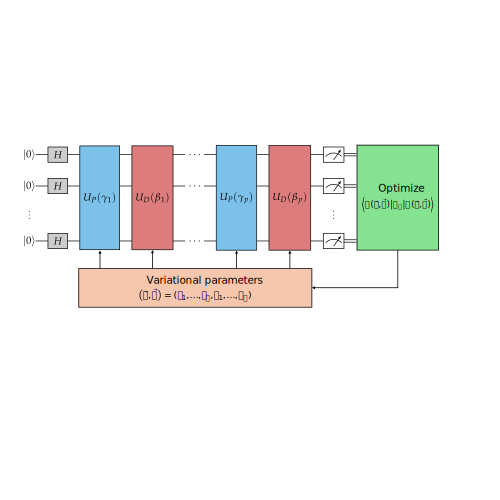
\includegraphics[width=0.9\textwidth]{figures/qaoa.pdf}
    \caption[Algorithme quantique d'optimisation approximative]{Schéma de l'algorithme quantique d'optimisation approximative (QAOA). Un circuit quantique paramétré est préparé en appliquant une alternance d'opérateurs de problème $U_{P}(\gamma)$ et de forçage $U_{D}(\beta)$ à un état initial $\ket{+}^{\otimes n}$. La valeur moyenne $\braket{ \psi(\vec{\gamma}, \vec{\beta}) | H_{P} | \psi(\vec{\gamma}, \vec{\beta}) }$ de l'Hamiltonien de problème $H_{P}$ est ensuite optimisée en modifiant les paramètres $\vec{\gamma}$ et $\vec{\beta}$ du circuit à l'aide d'un optimiseur classique.}
    \label{fig:qaoa}
\end{figure}

Décrivons maintenant plus en détail les mécanismes derrière QAOA: la préparation de l'état initial, l'encodage du problème dans un hamiltonien de problème ainsi que le choix de l'hamiltonien de forçage. L'initialisation et l'optimisation des paramètres du circuit sont décrites à la section~\ref{subsec:configuration-des-parametres}.

%-----------------------------------------------------------------------------%

\subsubsection{Préparation de l'état initial}
\label{subsec:preparation-de-etat-initial}

Comme QAA, le circuit quantique est initialement préparé dans l'état fondamental de l'hamiltonien de forçage pour garantir le théorème adiabatique. Cependant, la divergence de QAOA du calcul adiabatique implique qu'un autre état initial peut être choisi. Une alternative consiste à utiliser une solution approximative du problème comme état initial~\cite{eggerWarmstartingQuantumOptimization2021}. L'état initial peut aussi être choisi de manière à restreindre l'espace des solutions. Au lieu de l'état initial $\ket{\psi_{0}} = \ket{0}^{\otimes n}$, un espace ne représentant que les solutions faisables du problème peut être préparé, tel qu'exemplifié à la section~\ref{subsec:forcage-de-grover}.

%-----------------------------------------------------------------------------%

\subsubsection{Encodage du problème}
\label{subsec:encodage-probleme}

Comment est-ce qu'un problème d'optimisation combinatoire $\varphi(x)$ peut être encodé par un hamiltonien $H_{P}$? D'abord, les entrées $x$ du problème sont caractérisées par une fonction de coût $C(x)$, pénalisant les configurations selon le nombre de contraintes non respectées. Une entrée optimale est associée à un coût nul, alors qu'une entrée non optimale est associée à un coût positif selon sa proximité avec la solution. Résoudre le problème consiste alors à trouver l'entrée optimale, c'est-à-dire l'entrée $x^{*}$ minimisant la fonction de coût. L'hamiltonien de problème se définit à partir de la fonction de coût tel que
\begin{equation}
    H_{P} \ket{x} = C(x) \ket{x} \,.
\end{equation}
Cette équation implique que l'état fondamental de l'hamiltonien $H_{P}$ encode les solutions au problème donné. QAOA cherche ainsi à préparer l'état fondamental de $H_{P}$ comme il correspond à une superposition des solutions au problème $\varphi$. Le modèle d'Ising est fréquemment utilisé pour fournir un hamiltonien de problème décrivant la fonction de coût $C$. En effet, trouver l'état fondamental d'un modèle d'Ising constitue un problème \textsf{NP}-complet, ce qui signifie qu'il existe alors nécessairement une réduction entre ce problème et les différents problèmes \textsf{NP}-complet. Le modèle d'Ising est donné par
\begin{equation}
    \label{eq:hamiltonien-ising}
    H_P = - \sum_{(i,j) \in E} J_{ij} \sigma_i \sigma_j - \sum_{i \in V} h_i \sigma_i \,,
\end{equation}
où $E$ est l'ensemble d'arêtes, $V$ est l'ensemble de sommets et $\sigma_{i}$ est le spin du site $i$. Les constantes $J$ et $h$ représentent respectivement l'interaction entre deux sites et le champ magnétique externe. Le problème d'optimisation quadratique binaire non contraint (« Quadratic Unconstrained Binary Optimization ») (QUBO) permet aussi d'exprimer les fonctions de coût de manière plus générale, en ne les restreignant pas au modèle d'Ising.

\begin{figure}[h]
    \centering
    \includegraphics[width=0.6\textwidth]{figures/ising-mapping}
    \caption[Transformation du problème \#NAE3SAT et \#1-in-3SAT au modèle d'Ising]{Exemple de la transformation entre le modèle d'Ising pour NAE3SAT et 1-in-3SAT pour une formule $\varphi$. À gauche, le graphe de facteurs de $\varphi$ avec les sommets de variables (bleus) et de clauses (gris). À droite, le modèle d'Ising correspondant à $\varphi$. Pour 1-in-3SAT, un terme de champ magnétique est ajouté pour favoriser les configurations où chaque clause contient exactement une variable fixée à 1.}
    \label{fig:transformation-ising}
\end{figure}

La formulation de problèmes \textsf{NP}-complet sous la forme du modèle d'Ising n'est pas nécessairement évidente, mais plusieurs réductions ont été formulées pour le calcul adiabatique quantique~\cite{lucasIsingFormulationsMany2014,lodewijksMappingNPhardNPcomplete2020}. Une réduction intéressante dans notre cas relie le problème positif NAE3SAT au modèle d'Ising antiferromagnétique. Une formule CNF $\varphi$ peut être représentée graphiquement sous la forme d'un graphe biparti nommé \textit{graphe de facteurs}. Dans ce graphe, les clauses et les variables forment les deux types de sommets de la bipartition, alors que les arêtes sont définies entre les sommets de ces deux partitions et correspondent à la présence d'une variable dans une clause. Considérons pour le moment une seule clause $C = (x_{1} \lor x_{2} \lor x_{3})$ de $\varphi$ et montrons comment transformer celle-ci au modèle d'Ising. En associant chaque variable $x_{i}$ à un spin $\sigma_{i}$ selon la transformation $\sigma_{i} = 1 - 2x_{i}$, cette clause se réduit à un modèle d'Ising antiferromagnétique en considérant un réseau triangulaire composé des spins $\sigma_{i}$, où chacun de ceux-ci interagit avec les deux autres spins comme illustré à la figure~\ref{fig:transformation-ising}. L'hamiltonien du modèle d'Ising associé à la clause $C = (x_{1} \lor x_{2} \lor x_{3})$ est alors donné par
\begin{equation}
    H_{P, C}^{\text{NAE3SAT}} = \sigma_{1}\sigma_{2} + \sigma_{2}\sigma_{3} + \sigma_{3}\sigma_{1} \,.
\end{equation}
Pour valider cette transformation, l'énergie associée à chaque combinaison possible de spins est présentée dans le tableau~\ref{tab:energie-nae3sat}. La frustration des spins sur le réseau implique que les seuls états qui ne sont pas dans l'état fondamental sont les états $\ket{\uparrow \uparrow \uparrow}$ et $\ket{\downarrow \downarrow \downarrow}$. Or, il s'agit des deux combinaisons ne faisant pas partie de l'ensemble des solutions du problème positif NAE3SAT. L'état fondamental de l'hamiltonien $H_{P, C}$ correspond ainsi bien aux solutions de la clause $C$.

\begin{table}[h]
    \centering
    \begin{subtable}{0.49\textwidth}
        \centering
        \begin{tabular}{c c}
            \hline
            Entrées (spins) & Coût (énergie) \\
            \hline
            000 & 3 \\
            001 & -1 \\
            010 & -1 \\
            100 & -1 \\
            011 & -1 \\
            110 & -1 \\
            101 & -1 \\
            111 & 3 \\
            \hline
        \end{tabular}
        \caption{}
        \label{tab:energie-nae3sat}
    \end{subtable}
    \begin{subtable}{0.49\textwidth}
        \centering
        \begin{tabular}{c c}
            \hline
            Entrées (spins) & Cout (énergie) \\
            \hline
            000 & 0 \\
            001 & -2 \\
            010 & -2 \\
            100 & -2 \\
            011 & 0 \\
            110 & 0 \\
            101 & 0 \\
            111 & 6 \\
            \hline
        \end{tabular}
        \caption{}
        \label{tab:energie-1in3sat}
    \end{subtable}
    \caption{Coût de chaque entrée d'une clause $C = (x_{1} \lor x_{2} \lor x_{3})$ d'une formule CNF pour le problème NAE3SAT (a) et 1-in-3SAT (b). Ce coût correspond à l'énergie du modèle d'Ising donnée par l'hamiltonien $H_{P,C}$ pour une combinaison de spins, reliée aux entrées par la transformation $\sigma_{i} = 1 - 2x_{i}$.}
\end{table}

Une formule CNF est représentable par un modèle d'Ising en appliquant la transformation précédente sur chacune des clauses $C$ de la formule, tel qu'illustré à la figure~\ref{fig:transformation-ising}, donnant ainsi l'hamiltonien 
\begin{equation}
    H_{P} = \sum_{C} H_{P, C} \,.
\end{equation}
Cet hamiltonien impose alors les contraintes de chaque clause. Remarquons que l'hamiltonien de problème pour NAE3SAT est donné par l'hamiltonien d'Ising donné à l'équation~\ref{eq:hamiltonien-ising} avec $J_{ij}=-1$ et $h_{i}=0$ pour un graphe construit comme à la figure~\ref{fig:transformation-ising}. Similairement, le problème 1-in-3SAT se transforme au modèle d'Ising en ajoutant pour chaque clause l'hamiltonien
\begin{equation}
   H_{P, C}^{\text{1-in-3SAT}} = \sigma_{1}\sigma_{2} + \sigma_{2}\sigma_{3} + \sigma_{3}\sigma_{1} - \sigma_{1} - \sigma_{2} - \sigma_{3} \,.
\end{equation}
Un champ magnétique externe est ajouté sur chaque spin pour imposer la contrainte supplémentaire, c'est-à-dire que toutes les clauses doivent contenir exactement une variable évaluant à un vrai logique. Le tableau~\ref{tab:energie-1in3sat} présente les énergies des configurations pour l'hamiltonien précédent, validant la correspondance entre les états fondamentaux et les solutions du problème SAT. L'hamiltonien pour le problème 1-in-3SAT est ainsi donné par l'hamiltonien d'Ising donné à l'équation~\ref{eq:hamiltonien-ising} avec $J_{ij}=-1$ et $h_{i}=1$.

%-----------------------------------------------------------------------------%

\subsubsection{Choix du forçage}

L'hamiltonien de forçage $H_{D}$ initialement proposé avec QAOA prend son inspiration de l'algorithme adiabatique quantique, en utilisant l'hamiltonien facile à préparer $H_{D}^{X}$. Cela implique que toute la dépendance au problème doit être encodée dans l'hamiltonien de problème $H_{P}$. Comme QAOA n'est pas restreint par cette condition, des opportunités se présentent pour encoder différemment le problème. Par exemple, l'hamiltonien de forçage peut être utilisé pour restreindre l'espace de Hilbert en prenant en compte la structure du problème. Divers hamiltoniens offrent différentes performances selon le problème étudié. Le meilleur choix de forçage demeure toutefois une question ouverte.

%-----------------------------------------------------------------------------%

\subsection{Relation avec l'algorithme adiabatique quantique}
\label{subsec:discretisation-qaoa}

QAA requiert une évolution continue de l'état, alors que QAOA repose sur l'application de portes quantiques. Pour établir un lien entre QAA et QAOA, l'évolution de l'hamiltonien de QAA doit donc être rendue discrète. Pour ce faire, l'évolution unitaire de QAA est émulée avec des portes quantiques en décomposant l'opérateur d'évolution $U(t) = e^{-i \int_{0}^{T} H(t) dt}$ de l'hamiltonien de QAA en séquence de petits pas de temps~\cite{blekosReviewQuantumApproximate2024}, tel que
\begin{equation}
    \label{eq:discretisation-qaa}
    U(t) \approx \prod_{k=0}^{t / \Delta t -1} e^{-i H(k \Delta t) \Delta t} \,,
 \end{equation}
pour un intervalle de temps $\Delta t$. Par la suite, la décomposition de Suzuki-Trotter, donnée par $e^{(A+B)t} = \lim_{n \to \infty} (e^{At / n} e^{Bt / n})^{n}$ pour deux opérateurs $A$ et $B$, est employée. Le premier ordre de cette décomposition permet de discrétiser l'opérateur de l'hamiltonien dépendant du temps $H(t)=(1-\frac{t}{T})H_{D} + \frac{t}{T}H_{P}$ de QAA (voir l'équation~\ref{eq:chemin-adiabatique}), où $t \in [0, T]$, tel que
\begin{equation}
    e^{-i H(t) } \approx e^{-i (1 - \frac{t}{T}) H_D \Delta t} e^{-i \frac{t}{T} H_P \Delta t} + O(\Delta t^2) \,.
\end{equation}
La forme de l'opérateur d'évolution de QAOA pour une profondeur $p=1$ de circuit est retrouvée en prenant $\beta = (1 - \frac{t}{T}) \Delta t$ et $\gamma = (\frac{t}{T}) \Delta t$~\cite{sackQuantumAnnealingInitialization2021}. Combinant cette dernière équation avec l'équation~\ref{eq:discretisation-qaa}, l'opérateur d'évolution devient
\begin{equation}
    U(t) \approx \prod_{k=0}^{t / \Delta t -1} e^{-i (1 - \frac{k \Delta t}{T}) H_{D} \Delta t} e^{- i \frac{k \Delta t}{T} H_{P} \Delta t} \,.
 \end{equation}

 Ce processus est généralement nommé \textit{évolution adiabatique trottérisée} en référence à la décomposition de Suzuki-Trotter. Dans la limite $p \to \infty$, une évolution adiabatique est retrouvée, car la condition adiabatique est satisfaite. Pour un circuit de profondeur $p$ finie, plus les paramètres $\gamma$ et $\beta$ sont faibles, plus les erreurs découlant de la discrétisation, communément appelées \textit{erreurs de Trotter}, sont atténuées, car le pas de temps d'évolution est raccourci. Cependant, cela diminue aussi la durée totale d'évolution adiabatique $T$, augmentant ainsi l'impact des excitations diabatiques qui nuisent à la performance de l'algorithme. Au contraire, des paramètres plus grands allongent le temps d'évolution aux dépens de l'augmentation des erreurs de Trotter. Un compromis entre ces deux facteurs doit être choisi pour minimiser les erreurs.

%-----------------------------------------------------------------------------%

\section{Ansatz quantique à opérateurs alternants}
\label{sec:ansatz-quantique-a-operateurs-alternants}

L'algorithme quantique d'optimisation approximative applique en alternance des opérateurs basés sur l'hamiltonien de problème et l'hamiltonien de forçage, guidé par l'algorithme quantique adiabatique. Cet algorithme comporte une limitation importante: les opérateurs appliqués doivent prendre la forme d'une évolution temporelle d'un hamiltonien local fixe. Cette restriction entrave la construction d'opérateurs unitaires potentiellement plus efficaces.

L'\textit{ansatz quantique à opérateurs alternants} (« Quantum Alternating Operator Ansatz») (QAOA), introduit par Hadfield et coll.~\cite{hadfieldQuantumApproximateOptimization2019}, généralise l'algorithme quantique d'optimisation approximative en permettant l'alternance de familles générales d'opérateurs unitaires paramétrés plutôt qu'uniquement des opérateurs basés sur un hamiltonien. Notons qu'un \textit{ansatz} décrit typiquement une sous-routine composée d'une séquence de portes appliquées sur des qubits spécifiques. Cette approche supporte ainsi la représentation d'un plus grand nombre d'états, pouvant possiblement être construite de manière plus efficace. De plus, celle-ci facilite l'utilisation d'opérateurs plus facilement réalisables sur le matériel informatique quantique actuel. Cette extension trouve toutefois son utilité principale dans la création d'opérateurs de forçage. En effet, ces opérateurs peuvent désormais être construit de manière à restreindre l'espace des configurations d'un problème selon ses contraintes et ainsi éviter une recherche de l'espace de Hilbert complet. 

L'algorithme quantique d'optimisation approximative et l'ansatz quantique à opérateurs alternants possèdent le même acronyme. Comme cette dernière étend le premier, l'acronyme QAOA fera référence à l'ansatz quantique à opérateurs alternants pour le reste de la présente section.

%-----------------------------------------------------------------------------%

\subsection{Description de l'approche}

Soit un problème d'optimisation combinatoire $\varphi(x)$ et une fonction de coût $C(x)$ décrivant la qualité des entrées $x$ de $\varphi$. Généralisant l'algorithme de Farhi, Goldstone et Gutmann, QAOA est constitué de deux familles d'opérateurs: les opérateurs de séparation de phase $U_{P}(\gamma)$ et les opérateurs de forçage $U_{D}(\beta)$, où $\gamma$ et $\beta$ sont des paramètres réels. Notons que $U_{P}$ et $U_{D}$ ne sont pas restreints à la classe d'opérateurs $e^{-i \theta H}$. Le circuit QAOA est construit en appliquant en alternance $p$ couches d'opérateurs des deux familles précédentes à un état initial donné.
        
Plutôt que de prendre en compte l'espace de Hilbert complet, un \textit{sous-espace faisable} $F$ est considéré. Cet espace ne représente qu'un sous-ensemble de l'espace des configurations possibles, où seules les configurations respectant les contraintes du problème sont présentes. La restriction provient de la famille d'opérateurs de forçage encodant les différentes contraintes du problème $\varphi$. En général, l'état initial est construit à partir d'une solution faisable alors que l'opérateur de forçage s'assure de restreindre les états possibles au sous-espace faisable. QAOA est donc particulièrement utile pour les problèmes comportant des contraintes rigides. Par exemple, le problème de recouvrement de sommets maximal nécessite que les solutions prennent la forme d'un état de Dicke, c'est-à-dire une superposition de tous les états de même poids d'Hamming. Intuitivement, limiter l'espace des configurations devrait améliorer la performance de l'algorithme. 

Quelques restrictions sont appliquées dans la conception des composantes de QAOA. D'abord, l'état initial doit être trivial à réaliser, c'est-à-dire réalisable avec un circuit de profondeur constante. Les unitaires de séparation de phases doivent être diagonales dans la base computationnelle et sont prises dans la majorité des cas comme $U_{P}(\gamma) = e^{-i \gamma H_{P}}$. La construction des unitaires de forçage est ici d'un plus grand intérêt. Ceux-ci doivent préserver le sous-espace faisable et donc transformer les états faisables en états faisables. Les unitaires de forçage doivent aussi fournir des transitions entre toutes les paires d'états correspondant aux états faisables.

%-----------------------------------------------------------------------------%

\subsection{Forçage de Grover}
\label{subsec:forcage-de-grover}

\textit{L'ansatz quantique à opérateurs alternants avec forçage de Grover} (« Grover-Mixer Quantum Alternating Operator Ansatz ») (GM-QAOA) fut proposé par Bärtschi et Eidenbenz~\cite{bartschiGroverMixersQAOA2020} pour déplacer la complexité de la conception de l'opérateur de forçage à la préparation de l'état initial en s'inspirant de l'algorithme de Grover. Cet algorithme se base sur le cadre théorique défini dans la section précédente pour produire efficacement une superposition égale de toutes les solutions faisables.

Décrivons d'abord rapidement le circuit GM-QAOA, tel qu'illustré à la figure~\ref{fig:gm-qaoa}. Un opérateur unitaire de préparation d'état $U_{S}$ crée une superposition égale $\ket{F}$ de toutes les solutions faisables du sous-espace faisable $F$. Par la suite, similairement à QAOA, les opérateurs unitaires de problème $U_{P}$ et de forçage $U_{M}$ sont appliqués en alternance $p$ fois.

\begin{figure}[ht!]
    \centering
    \includegraphics[width=0.7\textwidth]{figures/gm-qaoa}
    \caption[Circuit de l'ansatz quantique à opérateurs alternants avec forçage de Grover]{Première couche du circuit de l'ansatz quantique à opérateurs alternants (GM-QAOA). Ce circuit est composé de l'opérateur de préparation d'état $U_{S}$, de l'opérateur de problème $U_{P}$, de portes de Pauli $X$ ainsi que d'une porte de déphasage $Z^{-\beta \pi}$ contrôlée sur tous les qubits. L'opérateur de forçage $U_{D}$ regroupe les opérateurs à l'intérieur de la boite pointillée.}
    \label{fig:gm-qaoa}
\end{figure}

Plutôt que de préparer un état initial à partir d'un état faisable, comme QAOA, l'état initial de GM-QAOA est préparé dans une superposition de l'entièreté des états faisables. Cette distinction entraine une perspective différente de celle adoptée par QAOA. La difficulté provient désormais de la préparation de l'état plutôt que de la conception de l'opérateur de mélange. L'opérateur de mélange $U_{D}$ quant à lui, est donné par
\begin{equation}
    U_D^{\mathrm{Grover}} = e^{-i \beta \ket{F}\!\bra{F}} = U_{S}\left[ \mathds{1}^{\otimes n} -\left(1-e^{-i \beta}\right) (\ket{0}\!\bra{0})^{\otimes n} \right] U_{S}^{\dagger} \,,
\end{equation}
où $U_{S}$ est l'opérateur de préparation d'état préparant l'état initial $\ket{F}$. L'opérateur $U_{D}^{\mathrm{Grover}}$ s'apparente aux opérateurs de diffusion utilisés dans l'algorithme d'amplification d'amplitude, où les opérateurs de déphasage $e^{-i\beta}$ remplacent les opérateurs d'inversion de phase $e^{-i \pi}$. $U_{D}$ est alors réalisé en utilisant les unitaires $U_{S}$ et $U_{S}^{\dagger}$, deux couches d'opérateur de Pauli $X$ et un opérateur de déphasage $Z^{-\beta/\pi} = \begin{pmatrix}
1 & 0 \\
0 & e^{-i\beta}
\end{pmatrix}$ contrôlés sur tous les qubits.

L'influence de l'algorithme de Grover sur GM-QAOA a notamment pour conséquence que GM-QAOA génère des superpositions uniformes d'états ayant la même énergie. Cette propriété est d'un intérêt particulier pour ce projet, comme elle garantit la distribution de solutions uniforme nécessaire à l'algorithme de JVV. De plus, comme cette approche est réalisable directement à partir d'un ensemble de portes quantiques standard, aucune erreur de simulation d'hamiltonien, comme les erreurs de Trotter, affecte l'algorithme. Notons que les problèmes NAE3SAT et 1-in-3SAT ne sont pas contraints et donc que l'espace faisable demeure le même que pour QAOA, c'est-à-dire que $\ket{F} = \ket{+}^{\otimes n}$.

%-----------------------------------------------------------------------------%

\section{Configuration des paramètres}
\label{subsec:configuration-des-parametres}

La capacité d'entraînement des réseaux de neurones à partir d'une simple descente de gradient fut en partie à l'origine de leur succès retentissant sur de nombreux différents problèmes. L'optimisation des paramètres se fait simplement, même avec des fonctions de coût non convexes, tout en offrant de puissants résultats. Une des attentes envers les VQA était qu'ils possèdent ce même comportement et qu'ils puissent ainsi repousser les limites des algorithmes variationnels. En effet, l'optimisation classique des paramètres de QAOA fait partie intégrante du concept d'algorithme variationnel quantique. Grâce à celle-ci, il est en théorie possible de tirer avantage des algorithmes quantiques en recourant à des ordinateurs quantiques bruités. Cependant, de nombreuses embûches rendent actuellement cette tâche difficile. 

D'abord, l'estimation du gradient de coût est difficile dans de nombreuses situations en raison de la présence de plateaux stériles~\cite{mccleanBarrenPlateausQuantum2018, laroccaReviewBarrenPlateaus2024}, où le gradient devient exponentiellement petit avec la taille du système. Un nombre exponentiel de mesures devient alors nécessaire pour pouvoir identifier la direction minimisant la fonction de coût. Ces complications se présentent surtout pour des circuits de grande profondeur, mais d'autres problèmes surgissent même pour ceux de petites tailles. Un grand nombre de minima locaux sont effectivement considérés comme pauvres, c'est-à-dire qu'ils possèdent une énergie petite par rapport au minimum global, augmentant la difficulté d'atteindre une solution approximative de bonne qualité~\cite{anschuetzQuantumVariationalAlgorithms2022}. De plus, l'optimisation des paramètres des VQA est \textsf{NP}-difficile, et donc intraitable dans le pire des cas~\cite{bittelTrainingVariationalQuantum2021}. Ces difficultés sont d'autant plus importantes comme la complexité de l'espace des paramètres augmente avec le nombre de paramètres d'un circuit, ce qui implique une plus grande difficulté d'optimisation pour les circuits profonds. 

Cet ensemble de complications implique alors qu'une bonne initialisation des paramètres est nécessaire au succès de QAOA. Des paramètres initiaux suffisamment près de l'extremum global peuvent aider à contourner les problèmes énoncés précédemment. Le choix de bons paramètres demeure toutefois une question ouverte. Parmi les différentes approches, Sack et Serbyn proposent une stratégie d'initialisation basée sur le \textit{recuit quantique trottérisé} (« Trotterized Quantum Annealing ») (TQA)~\cite{sackQuantumAnnealingInitialization2021}. Cette méthode, utilisée pour les simulations de ce travail, offre la même performance qu'un nombre exponentiel d'initialisations aléatoires. Comme vu à la section~\ref{subsec:discretisation-qaoa}, un juste milieu doit être choisi entre le temps d'évolution et les erreurs de Trotter. L'initialisation TQA permet de trouver le temps d'évolution optimal à une profondeur de circuit $p$ fixe. Pour ce faire, la procédure décrite à la section~\ref{subsec:discretisation-qaoa} est appliquée sur une grille uniformément discrétisée des temps d'évolution $t_{k} = k \Delta t$, avec $k = 1,\dots, p$, pour un pas de temps $\Delta t = T / p$. Les angles du circuit QAOA correspondant sont alors:
\begin{equation}
    \gamma_{i} = \frac{i}{p} \Delta t \,, \beta = (1 - \frac{i}{p}) \Delta t \,.
\end{equation}
Le pas de temps est optimisé classiquement en mesurant la valeur moyenne de l'hamiltonien de problème $H_{P}$ de manière à minimiser cette dernière, donnant ainsi de bons paramètres initiaux.

%-----------------------------------------------------------------------------%

\section{Échantillonnage et biais}
\label{sec:echantillonnage-et-biais}

L'allure de la distribution obtenue par QAOA est dans notre cas essentiel. Afin de se conformer à la condition de l'algorithme de JVV, celle-ci doit être quasi uniforme, c'est-à-dire qu'elle doit posséder une faible non-uniformité. Est-ce le cas? D'abord, à moins que l'état préparé soit optimal, des non-solutions sont nécessairement présentes dans la distribution obtenue, bien que potentiellement avec une faible probabilité. Comme l'algorithme de JVV nécessite une distribution constituée uniquement de solutions, cela pose problème. Une étape de post-sélection est alors nécessaire pour retirer les non-solutions des échantillons mesurés. Heureusement, vérifier la validité d'une entrée se fait efficacement pour les problèmes \textsf{NP}. Toutefois, rien ne nous garantit que la distribution restante, composée uniquement de solutions, est effectivement non-uniforme.

En général, le recuit quantique n'échantillonne pas les états fondamentaux uniformément~\cite{matsudaGroundstateStatisticsAnnealing2009, mandraExponentiallyBiasedGroundState2017}. Certains états sont exponentiellement supprimés et nécessitent un nombre exponentiel de mesures pour être détectés. Comme le recuit quantique et QAOA sont fortement liés, il est ainsi peu probable que QAOA puisse échantillonner les états fondamentaux de manière uniforme.

Une propriété de l'algorithme GM-QAOA devient alors d'un intérêt considérable: l'équiprobabilité des états de même énergie. Les solutions étant encodées dans l'état fondamental de l'hamiltonien de problème, elles possèdent ainsi la même amplitude et donc la même probabilité. En ne considérant que les solutions, l'état préparé par le circuit GM-QAOA possède toujours une non-uniformité nulle, un avantage non négligeable par rapport à QAOA.


\chapter{Comptage variationnel quantique}
\label{cha:comptage-variationnel-quantique}

%-----------------------------------------------------------------------------%

\begin{comment}
\subsection*{Plan}

\begin{enumerate}
    \item Expliquer que cette section ne concerne que GM-QAOA
\end{enumerate}
\end{comment}

Les chapitres précédents ont laissés transparaître l'intuition derrière l'approche empruntée dans ce travail: Est-il possible d'utiliser les algorithmes variationnels comme générateur de solutions à l'algorithme de JVV pour la résolution approximative des problèmes de comptage? Avant d'introduire le fruit du travail de ce mémoire, l'algorithme VQCount, énumérons les difficultés liées à la résolution de problèmes de comptage avec les algorithmes variationnels quantiques. D'abord, les circuits quantiques doivent produire une grande séparation entre les amplitudes des solutions et les non-solutions de l'état produit pour pouvoir produire même une seule solution avec un nombre tractable de mesures. Ensuite, même si les amplitudes des non-solutions sont nulles, si les amplitudes d'un sous-ensemble non négligeable des solutions sont significativement supprimés par rapport aux autres amplitudes, la mesure des états supprimés entraîne une surcharge computationnelle, potentiellement exponentielle, du nombre de répétitions. Finalement, même si toutes les solutions possèdent environ des amplitudes égales et si les non-solutions ne sont pas présentes dans l'état produit, un nombre exponentiel de mesures est en théorie nécessaire pour énumérer naïvement les solutions de manière exhaustive comme le nombre de solutions est exponentiel pour les problèmes d'intérêt.

L'apport principal de ce travail réside dans la combinaison des algorithmes variationnels quantique et l'algorithme de JVV. L'algorithme VQCount échantillonne la distribution préparée par un algorithme variationnel quantique afin de produire un compte approximatif à l'aide de l'algorithme de JVV. Cette approche tente de minimiser l'impact des obstacles précédents, en particulier la deuxième et troisième difficulté. L'utilisation de GM-QAOA permet d'éviter la suppression d'amplitude d'un sous-ensemble de solutions en assurant que toutes les solutions aient la même amplitude. De plus, l'algorithme de JVV prend avantage de la structure des problèmes auto-réductibles pour éviter de devoir énumérer naïvement toutes les solutions. 

Ce chapitre débute en introduisant l'algorithme VQCount à la section~\ref{sec:algorithme-vqcount} et décrit la procédure d'auto-réduction nécessaire à l'algorithme VQCount à la section~\ref{sec:procedure-auto-reduction}.

%-----------------------------------------------------------------------------%

\section{Algorithme VQCount}
\label{sec:algorithme-vqcount}

\begin{comment}
\subsection*{Plan}

\begin{enumerate}
    \item Vulgariser l'algorithme de manière général
    \item Expliquer rigoureusement l'algorithme
    \item Faire le lien entre la notation utilisée dans les algorithmes de comptage classique
    \item Faire la comparaison avec les travaux précédents
    \item Rajouter l'algorithme complet en pseudo-code
\end{enumerate}

\subsection*{Références}
\end{comment}

Comment faire le pont entre les algorithmes variationnels quantiques et l'algorithme de JVV pour la résolution de problème de comptage? A priori, l'algorithme de JVV doit tout simplement être implémenté en utilisant un algorithme variationnel quantique comme générateur de solutions. Cependant, plusieurs embûches barrent notre chemin. Décrivons la procédure, nommé VQCount par brièveté, en affrontant ces problèmes en chemin.

Soit une instance de problème SAT, décrite par la formule CNF $\varphi$. Ce problème est auto-réductible par la relation~\ref{rel:auto-reductibilite-sat}. Ce travail se limite à l'étude du problème SAT en gardant en tête que par sa \textsf{NP}-complétude, une réduction existe entre n'importe quel problème de la classe \textsf{NP} et celui-ci. La formule $\varphi$ peut être transformée en un modèle d'Ising, tel que décrit à la section~\ref{subsec:encodage-probleme}, de l'hamiltonien du modèle d'Ising $H_{P}$ encode le problème. Grâce à cet hamiltonien de problème, il est possible de construire le circuit paramétré quantique de l'algorithme QAOA, préparant l'état $\ket{\psi(\vec{\gamma}_{0}, \vec{\beta}_{0})}$ avec les paramètres initiaux $\vec{\gamma}_0$ et $\vec{\beta}_{0}$. Négligeons pour le moment le choix de l'état initial et de l'hamiltonien de forçage. Une fois le circuit construit, l'énergie moyenne de $H_{P}$ est évalué à l'aide de mesures répétées de l'état préparé. Un optimiseur classique modifie ensuite les paramètres du circuit quantique pour minimiser cette énergie, donnant un circuit quantique paramétré optimisé $\ket{\psi(\vec{\gamma}, \vec{\beta})}$.
Les échantillons, obtenus par une mesure dans la base computationnelle de l'état préparé par le circuit, contient alors, avec une haute probabilité, des solutions à la formule $\varphi$.

QAOA étant une méthode heuristique, les paramètres optimaux ne sont pas nécessairement atteints, impliquant la présence de non-solutions dans la distribution obtenue en mesurant $\ket{\psi(\vec{\gamma}, \vec{\beta})}$. L'algorithme de JVV nécessite pourtant une distribution composée uniquement de solutions, impliquant qu'une étape de post-traitement doit être employé pour retirer les non-solutions. Comme le problème SAT appartient à la classe \textsf{NP}, vérifier qu'un échantillon est une solution est un processus efficace. Ainsi, toutes les non-solutions échantillonnées sont retirées de la distribution obtenue. De plus, comme discuté à la section~\ref{sec:echantillonnage-et-biais}, la non-uniformité de la distribution obtenue ne respecte pas nécessairement la condition de l'algorithme de JVV. La discussion dans cette section se restreindra alors à la variante GM-QAOA, qui garantie que les amplitudes des solutions préparées soient égales. Ainsi, le critère de mérite pertinent est la probabilité que le résultat d'une mesure soit une solution, ou plus succinctement le \textit{taux de succès}:

\begin{equation}
    r = \braket{ \psi(\vec{\gamma}, \vec{\beta}) | \hat{\mathcal{P}}_{G} | \psi(\vec{\gamma}, \vec{\beta}) }
\end{equation}

où $\hat{\mathcal{P}}_{G}$ est le projecteur dans l'espace des solutions $G$, c'est-à-dire l'état fondamental du modèle d'Ising représentant le problème, donné par

\begin{equation}
    \hat{\mathcal{P}}_{G} = \sum_{x \in G} \ket{x}\!\bra{x}
\end{equation}

Cette définition permet alors de décrire la performance des différents algorithmes pour le comptage basé sur l'échantillonnage sur un pied d'égalité en utilisant le taux de succès $r$, la tolérance (ou l'erreur multiplicative) $\varepsilon$ ainsi que la confiance $\delta$. Cette caractérisation s'étend aux algorithmes classiques employant un générateur échouant à produire une solution à un taux $1 - r$.

Ces remarques complétées, des échantillons sont mesurés à partir du circuit $\ket{\vec{\gamma}, \vec{\beta}}$ pour estimer la valeur la plus probable de la première variable $w_{0}$. Selon l'algorithme de JVV, il faut alors échantillonner des solutions à la sous-instance $\varphi_{w_{0}}$. Résoudre directement celle-ci à l'aide du même circuit optimisé demanderait une post-sélection supplémentaire sur la première variable. En réalité, comme il existe un nombre exponentiel de sous-instances en raison du nombre exponentiel de chaînes de bits possibles, un nombre exponentiel d'échantillons supplémentaires devraient être retiré. Une autre méthode consiste à construire et optimiser un différent circuit pour résoudre la sous-instance. Pour éviter cette surcharge computationnelle, le circuit de GM-QAOA est modifié pour résoudre directement la sous-instance. Cette procédure d'auto-réduction, qui consiste à remplacer pour chaque qubit fixé la porte d'Hadamard par une porte de Pauli conditionnée sur la valeur $w_{0}$ du bit fixé et à retirer l'opérateur de l'hamiltonien de forçage sur le qubit associé, est détaillée à la section~\ref{sec:procedure-auto-reduction}.
Ce changement permet de conserver la propriété d'égalité des amplitudes de GM-QAOA. De plus, celle-ci suggère qu'il soit possible d'éviter d'optimiser à nouveau le circuit en gardant les mêmes paramètres. Ainsi, le circuit est modifié selon la procédure d'auto-réduction sans optimiser les paramètres. Des solutions sont alors encore échantillonnées de ce sous-circuit et le processus est répété de manière récursive jusqu'à ce que toutes les variables soient fixées. Le nombre de solutions est alors données par l'inverse du produit des probabilités conditionnelles tel qu'énoncé par l'algorithme de JVV. L'algorithme~\ref{alg:algorithme-jvv} résume les étapes de l'algorithme VQCount.

\begin{algorithm}[h!]
    \caption{VQCount}\label{alg:vqcount}
    \begin{algorithmic}[1]
    \REQUIRE Nombre de variables: $n$, Hamiltonien de problème: $H_P$,\\Hamiltonien de forçage: $H_D$, Paramètres initiaux: $(\vec{\beta}_0, \vec{\gamma}_0)$, Profondeur: $p$, Nombre d'étapes d'optimisation: $n_{o}$, Nombre de solutions à\\échantillonner: $n_s$
    
    \STATE PQC($\vec{\beta}_0, \vec{\gamma}_0) \leftarrow \text{Circuit-QAOA}(H_P, H_D, \vec{\beta}_0, \vec{\gamma}_0, p$)
    \STATE $\text{PQC}(\vec{\beta}, \vec{\gamma}) \leftarrow \text{Optimisation}(\text{PQC}(\vec{\beta}_0, \vec{\gamma}_0), n_{o})$
    \STATE $w \leftarrow \texttt{""}$ 
    \STATE $\tilde{N} \leftarrow 1$
    \FOR{$i \in \{1, \dots, n\}$}
    \STATE $S \leftarrow \{ \ \}$
    \WHILE{$\abs{S} < n_{s}$}
    \STATE $m \leftarrow \text{Mesure}(\text{PQC}(\vec{\beta}, \vec{\gamma}))$
    \IF{$\text{Vérification-Solution}(m)$}
    \STATE $S \leftarrow S \cup \{m\}$
    \ENDIF
    \ENDWHILE
    \STATE $w, \tilde{p} \leftarrow \text{Préfixe-Majoritaire}(S)$
    \STATE $\text{PQC}(\vec{\beta}, \vec{\gamma}) \leftarrow \text{Auto-Réduction}(\text{PQC}(\vec{\beta}, \vec{\gamma}), w)$
    \STATE $\tilde{N} \leftarrow \tilde{N} / \tilde{p}$
    \ENDFOR
    
    \RETURN $\tilde{N}$
\end{algorithmic}
\end{algorithm}
    
Comme l'algorithme VQCount se fonde sur l'algorithme de JVV, son utilisation requiert $O(\frac{n^{2} \log (\frac{1}{\delta})}{r \varepsilon^{2}})$ échantillons pour approximer le nombre d'états fondamentaux à une erreur multiplicative $\varepsilon$ avec une confiance $1 - \delta$. Ce résultat se compare favorablement à un travail similaire évaluant la fonction de partition d'hamiltoniens de spin classiques qui requiert $O(\frac{\sqrt{N \log(1 / \delta)}}{r \varepsilon})$ échantillons pour la même tâche~\cite{sundarQuantumAlgorithmCount2019}. Lorsque $N=O(2^{n})$, VQCount nécessite exponentiellement moins d'échantillons que cette méthode.

Malgré que l'approche présentée résoute certains des problèmes énoncés au début de la section, les problèmes \textsf{\#P}-difficile demeure difficile pour les ordinateurs quantiques. La génération des distributions arbitraires, incluant les distributions uniformes de structures combinatoires, est difficile en général et seulement facile dans des cas exceptionnels~\cite{aaronsonComputationalComplexityLinear2011, boulandComplexityVerificationQuantum2019}. De plus, GM-QAOA requiert en général des profondeurs de circuits de taille exponentielle selon la taille du problème pour atteindre un taux de succès fini~\cite{xiePerformanceUpperBound2025}. 

Notons qu'un algorithme classique peut être utilisé pour résoudre l'instance du problème de comptage lorsque VQCount ait suffisamment réduit celle-ci.

% \begin{enumerate}[(1)]
%     \item \textbf{Auto-réductibilité:} Le problème de comptage doit être auto-réductible.
%     \item \textbf{Générateur de solutions:} Le générateur de solutions doit être en mesure de retourner des solutions pour toutes les sous-instances du problème.
%     \item \textbf{Non-uniformité:} Le générateur de solutions doit être quasi uniforme, c'est-à-dire dont la distribution de solutions tend vers l'inverse du nombre de variables.
% \end{enumerate}




%-----------------------------------------------------------------------------%

\section{Procédure d'auto-réduction}
\label{sec:procedure-auto-reduction}

\begin{comment}
\subsection*{Plan}
    \begin{enumerate}
    \item Faire la preuve de l'auto-réductibilité des algorithmes variationnels quantiques
\end{enumerate}
\end{comment}

% % \begin{figure}[h!]
% %     \centering
% %     \begin{quantikz}[font=\sffamily]
% %       \ket{0} & \gate[style={fill=mysilver!80}][0.80cm]{H} & \gate[wires=4, nwires=3, style={fill=myblue}][1.30cm]{U_P (\gamma_{1})} & \gate[wires=4, nwires=3, style={fill=myred}][1.30cm]{U_D (\beta_{1})} & \ \ldots\ \qw & \gate[wires=4, nwires=3, style={fill=myblue}][1.30cm]{U_P (\gamma_{p})} & \gate[wires=4, nwires=3, style={fill=myred}][1.30cm]{U_D (\beta_{p})} & \qw \\
% %       \ket{0} & \gate[style={fill=mysilver!80}][0.80cm]{H} & & & \ \ldots\ \qw & & & \qw \\
% %       \vdots & & & & & & & \\
% %       \ket{0} & \gate[style={fill=mysilver!80}][0.80cm]{H} & & & \ \ldots\ \qw & & & \qw
% %     \end{quantikz}
% %     \caption{}
% % \end{figure}



% % \begin{figure}[h!]
% %     \centering
% %     \begin{quantikz}
% %       \ket{0} & \gate[style={fill=myyellow!80}][0.80cm]{X^{c}} & \gate[wires=4, nwires=3, style={fill=myblue}][1.30cm]{U_P (\gamma_{1})} & \qw & \ \ldots\ \qw & \gate[wires=4, nwires=3, style={fill=myblue}][1.30cm]{U_P (\gamma_{p}) } & \qw & \qw \\
% %       \ket{0} & \gate[style={fill=mysilver!80}][0.80cm]{H} & & \gate[wires=3, nwires=2, style={fill=myred}][1.30cm]{U_D (\beta_{1})} & \ \ldots\ \qw & & \gate[wires=3, nwires=2, style={fill=myred}][1.30cm]{U_D (\beta_{p})} & \qw \\
% %       \vdots & & & & & & & \\
% %       \ket{0} & \gate[style={fill=mysilver!80}][0.80cm]{H} & & & \ \ldots\ \qw & & & \qw
% %     \end{quantikz}
% %     \caption{}
% % \end{figure}

% \begin{figure}[h!]
%     \centering
%     \begin{quantikz}[font=\sffamily]
%       \ket{0} & \gate[style={fill=mysilver!80}][0.80cm]{H} & \gate[wires=4, nwires=3, style={fill=myblue}][1.30cm]{U_P (\gamma_{1})} & \gate[wires=4, nwires=3, style={fill=myred}][1.30cm]{U_D (\beta_{1})} & \ \ldots\ \qw & \gate[wires=4, nwires=3, style={fill=myblue}][1.30cm]{U_P (\gamma_{p})} & \gate[wires=4, nwires=3, style={fill=myred}][1.30cm]{U_D (\beta_{p})} & \qw \\
%       \ket{0} & \gate[style={fill=mysilver!80}][0.80cm]{H} & & & \ \ldots\ \qw & & & \qw \\
%       \vdots & & & & & & & \\
%       \ket{0} & \gate[style={fill=mysilver!80}][0.80cm]{H} & & & \ \ldots\ \qw & & & \qw
%     \end{quantikz}
%     \caption{}
% \end{figure}

% \begin{figure}[h]
%     \centering
%     \begin{quantikz}
%         \ket{x_1} & \ctrl{3} & \qw      & \qw      & \qw      & \qw      & \qw      & \qw      & \qw      & \qw      & \qw      & \qw      & \qw     & \ctrl{3} & \qw \\
%         \ket{x_2} & \qw      & \ctrl{2} & \ctrl{3} & \qw      & \qw      & \qw      & \qw      & \qw      & \qw      & \qw      & \ctrl{3} & \ctrl{2}     & \qw      & \qw \\
%         \ket{x_3} & \qw      & \qw      & \qw      & \ctrl{2} & \qw      & \qw      & \qw      & \qw      & \qw      & \ctrl{2} & \qw      & \qw     & \qw      & \qw \\
%         \ket{0}   & \targ{}  & \targ{}  & \qw      & \qw      & \targ{}  & \ctrl{2}      & \qw      & \ctrl{2} & \targ{}  & \qw      & \qw      & \targ{}      & \targ{}  & \qw \\
%         \ket{0}   & \qw      & \qw      & \targ{}  & \targ{}  & \targ{}  & \ctrl{1}      & \qw     & \ctrl{1}  & \targ{}  & \targ{}  & \targ{}  & \qw     & \qw     & \qw \\
%         \ket{0}   & \qw      & \qw      & \qw      & \qw      & \qw      & \targ{}       & \ctrl{7} & \targ{}  & \qw      & \qw      & \qw      & \qw     & \qw      & \qw \\ [0.5cm]
%         \ket{x_4} & \ctrl{3} & \qw      & \qw      & \qw      & \qw      & \qw      & \qw      & \qw      & \qw      & \qw      & \qw      & \qw     & \ctrl{3} & \qw \\
%         \ket{x_5} & \qw      & \ctrl{2} & \ctrl{3} & \qw      & \qw      & \qw      & \qw      & \qw      & \qw      & \qw      & \ctrl{3} & \ctrl{2}     & \qw      & \qw \\
%         \ket{x_6} & \qw      & \qw      & \qw      & \ctrl{2} & \qw      & \qw      & \qw      & \qw      & \qw      & \ctrl{2} & \qw      & \qw     & \qw      & \qw \\
%         \ket{0}   & \targ{}  & \targ{}  & \qw      & \qw      & \targ{}  & \ctrl{2}      & \qw      & \ctrl{2} & \targ{}  & \qw      & \qw      & \targ{}      & \targ{}  & \qw \\
%         \ket{0}   & \qw      & \qw      & \targ{}  & \targ{}  & \targ{}  & \ctrl{1}      & \qw     & \ctrl{1}  & \targ{}  & \targ{}  & \targ{}  & \qw     & \qw     & \qw \\
%         \ket{0}   & \qw      & \qw      & \qw      & \qw      & \qw      & \targ{}       & \ctrl{1} & \targ{}  & \qw      & \qw      & \qw      & \qw     & \qw      & \qw \\ [0.5cm]
%         \ket{0}   & \qw      & \qw      & \qw      & \qw      & \qw      & \qw      & \gate{Z^{- \gamma \varepsilon/\pi}}  & \qw & \qw & \qw & \qw & \qw & \meter{} & \qw \\
%         \end{quantikz}
%     \caption{}
%     \label{fig:..}
% \end{figure}

Pour agir en tant que générateur de solutions à sous-instance de l'instance du problème original, le circuit GM-QAOA doit être modifié pour être en mesure d'échantillonner à partir de la distribution de solutions appropriée. Comme expliqué à la section précédente, il n'est pas suffisant d'échantillonner l'état produit par le circuit original en raison du nombre exponentielle de mesures nécessaires. Une \textit{procédure d'auto-réduction}, illustrée à la figure~\ref{fig:vqcount-circuit}, est ainsi introduite pour résoudre cette complication. Soit une formule CNF $\varphi$ et une sous-formule CNF $\varphi_{w}$ représentant la formule $\varphi$ où les premières variables sont remplacées par $w$. Alors, pour chaque qubit $q$ fixé à $w_{q}$ du circuit GM-QAOA, les opérations suivantes sont appliquées:

\begin{enumerate}[(1)]
    \item Retirer la porte d'Hadamard $H$ initiale du qubit $q$.
    \item Insérer un porte de Pauli $X$ conditionnée par la valeur $w_{q}$.
    \item Retirer l'opérateur de l'hamiltonien de forçage $H_{D}$ du qubit $q$.
\end{enumerate}

Ces modifications fixent alors l'état du qubit $q$ à $\ket{w_{q}}$ tout en préservant les termes d'interactions encodant les contraintes de la formule $\varphi_{w}$. De plus, le circuit modifié possède les propriétés de GM-QAOA. L'annexe~\ref{ann:auto-reductibilite-du-circuit-gm-qaoa} prouve la validité de ces affirmations.

\begin{figure*}[h!]
    \centering
    \begin{subfigure}[h]{0.6\textwidth}
    \centering
    \caption{}
    \includegraphics[width=1\textwidth]{figures/qaoa-self-reducibility-1.pdf}
    \label{fig:vqcount-circuit-a}
    \end{subfigure}
    \begin{subfigure}[h]{0.6\textwidth}
    \centering
    \caption{}
    \includegraphics[width=1\textwidth]{figures/qaoa-self-reducibility-2.pdf}
    \label{fig:vqcount-circuit-b}
    \end{subfigure}
\caption[Procédure d'auto-réduction de VQCount]{Générateur de solutions QAOA avant (a) et après (b) avoir fixé le premier qubit à $c$ durant la procédure d'auto-réduction.}
\label{fig:vqcount-circuit}
\end{figure*}

L'algorithme VQCount ne comprend qu'une optimisation des paramètres du circuit quantique paramétré avant la procédure d'auto-réduction. Toutefois, un autre cycle d'optimisation est en principe nécessaire pour chaque circuit réduit afin d'atteindre un état optimal représentant les solutions à la sous-instance du problème. Ce choix mène alors à la question suivante: Est-ce que la probabilité de succès $r$ du circuit réduit est égale ou supérieur à celle du circuit original avec les mêmes paramètres? Dans ce cas, l'optimisation n'est nécessaire que pour le circuit original et peut être sautée pour les circuits réduits.

La réponse à cette question est positive dans le cas de circuits GM-QAOA peu profonds dans la limite $\gamma_{i}=\beta_{i}$, $i=1,\dots,p$. Dans cette limite, GM-QAOA se réduit à l'algorithme de Grover. En effet, pour tous les hamiltoniens de problème $H_{P}$ pouvant être écrit comme une somme de chaînes de Pauli, un circuit peut être construit effondrant tous les niveaux excités de $H_{P}$ à un seul niveau excité, menant à circuit d'évolution d'hamiltonien à deux niveaux $U_{P}$. Avec les paramètres susmentionnés, $U_{P}$ devient un oracle pour les états fondamentaux de $H_{P}$, à une phase constante près, et $U_{D}$ devient l'opérateur de diffusion de Grover. Dans cette limite, à une profondeur constante $p=O(1)$, le taux de succès est une fonction strictement croissante du rapport des solutions au nombre total d'états. Si, en descendant l'arbre d'auto-réductibilité de l'algorithme de JVV, nous choisissons les branches possédant une probabilité plus grande que $1/2$, alors le ratio des solutions au nombre total d'états est aussi strictement croissant. Cela signifie que, pour ce choix de paramètres, un circuit GM-QAOA peu profond pour un problème donné peut être modifié selon la procédure d'auto-réduction pour résoudre les sous-problèmes avec le même ou un meilleur taux de succès. Cet argument est seulement valide dans la limite de Grover, mais suggère que la stratégie d'auto-réduction est possiblement aussi valide dans d'autres cas. Le chapitre suivant introduit des évidences sous la forme de simulations numériques pour confirmer la validité de cette intuition.

\begin{figure*}[h]
    \centering
    \includegraphics[width=0.7\textwidth]{figures/tower-of-excited-states.pdf}
    \caption{}
    \label{fig:tower-of-excited-states}
\end{figure*}

%-----------------------------------------------------------------------------%

% \section{Module VQCount}
% \label{sec:module-vqcount}

% \begin{comment}
% \subsection*{Plan}
% \begin{enumerate}
%     \item Expliquer les librairies python dévelopées
%     \item Décrire \textit{qaoa-quimb}
%     \item Décrire \textit{VQCount}
% \end{enumerate}
% \end{comment}



\begin{comment}
- Gibs phenomenon
- Post-processing used (how impactful is removing non-distinct solutions?)
- How does clean TVD evolve with JVV steps (see proof)?
- Approximation ratio
- Numerical analysis (which mean to take)
\end{comment}

\chapter{Résolution de problèmes \textsf{\#P}-complet avec VQCount}

%-----------------------------------------------------------------------------%

\begin{comment}
\subsection*{Plan}

\begin{enumerate}
    \item Mentionner les problèmes étudiés
    \item Mentionner les méthodes utilisées (réseaux de tenseurs)
    \item Décrire les paramètres de l'étude (nombre d'instances, régimes de complexité, etc.)
    \item Expliquer les principaux résultats (compromis entre QAOA et GM-QAOA)
\end{enumerate}

\subsection*{Références}
\end{comment}

Dans la section précédente, un cadre théorique s'appuyant sur l'algorithme de JVV a été construit pour la résolution de problèmes de comptage à l'aide d'algorithmes variationnels quantiques. L'algorithme résultant, VQCount, obtient un compte approximatif à une erreur multiplicative près en échantillonnant un nombre polynomial de solutions à un circuit quantique optimisé GM-QAOA. Toutefois, plusieurs conditions potentiellement dispensables ou difficilement applicables ont été imposées. Cette section change l'optique précédente en évaluant l'algorithme VQCount uniquement en tant que méthode heuristique, c'est-à-dire en caractérisant l'algorithme sans se soucier des garanties. la résolution de deux problèmes \textsf{\#P}-complet, \#NAE3SAT et \#1in3SAT, sont étudiés.

%-----------------------------------------------------------------------------%

\section{Paramètres de l'étude}


Certaines précédentes considérations sont ainsi relâchées ou modifiées. D'abord, l'algorithme GM-QAOA n'est plus considéré dans sa forme limite de Grover. Les paramètres $(\vec{\alpha}, \vec{\beta})$ sont optimisées plutôt que d'utiliser des paramètres fixes. De plus, les problèmes étudiés sont transformé à des Hamiltonians de problème régulier contenant une tour d'états excités plutôt que de l'oracle à deux niveaux construits précédemment.

L'algorithme VQCount est appliqué aux problèmes \#NAE3SAT positif et \#1-in-3SAT positif présentés à la section~\ref{sec:satisfaisabilite-booleenne}. Le problème \#NAE3SAT est difficile près du seuil de satisfaisabilité situé au ratio de clauses sur variables critique $\alpha_{c} \approx 2.1$. Pour étudier l'effet de la complexité des formules aléatoires sur la performance de VQCount, des instances sont générées à $\alpha = 1$ et $\alpha = 2$. Celles-ci sont générées à partir de graphes connectés biparties, imposant une restriction supplémentaire. Similairement, les instances du problème \#1-in-3SAT positive sont à leur seuil de difficulté le plus élevé près de $\alpha_{c} \approx 2/3$. Pour étudier ce problème dans le régime difficile, les instances sont générées à partir de graphes aléatoires cubiques, en plaçant une clause sur tous les sommets et une variable sur toutes les arrêtes. Ce type de problème appartient à la catégorie des problèmes verrouillés, décrit à la section~\ref{sec:transitions-de-phase}, étant vraisemblablement les plus plus difficiles des problèmes \#P. Par la suite, les instances générées sont convertis en un modèle d'Ising à l'aide de la transformation décrite à la section~\ref{subsec:encodage-probleme}.

La simulation de circuits quantiques est un problème complexe en raison de la quantité de mémoire nécessaire pour représenter l'espace d'Hilbert. La méthode la plus utilisée, la simulation à vecteur d'état, ne peut atteindre plus d'une vingtaine de qubits pour cette raison. Les réseaux de tenseur sont un outil alternatif puissant, particulièrement pour l'étude de circuits quantiques peu profonds. L'annexe~\ref{cha:reseaux-de-tenseurs} introduit les réseaux de tenseur et les méthodes particulières utilisées pour la simulation de l'algorithme VQCount. La librairie « Quimb »~\cite{grayQuimbPythonPackage2018} est utilisé pour modéliser l'optimisation et l'échantillonnage des circuits quantiques QAOA et GM-QAOA. Les paramètres de ces circuits sont optimisés avec la programmation séquentielle des moindres carrés tel qu'implémenté par la librairie « SciPy »~\cite{virtanenSciPy10Fundamental2020}. Pour évaluer la validité des résultats obtenus, « Ganak »~\cite{sharmaGANAKScalableProbabilistic2019}, un compteur de modèles exact basé sur une approche probabiliste, est utilisé pour trouver le nombre exact de solutions et le solveur SAT « Glucose3 »~\cite{eenExtensibleSATsolver2004,audemardPredictingLearntClauses2009} , implémenté dans l'ensemble d'outils « PySAT »~\cite{ignatievPySATPythonToolkit2018}, est utilisé pour énumérer toutes les solutions.

Pour le problème \#NAE3SAT, 20 instances aléatoires sont générées par taille d'instance, allant de 6 à 20 variables, pour les deux densités de clause $\alpha=1$ et $\alpha = 2$. Similairement, problème \#1-in-3SAT, 20 instances aléatoires sont générées pour une taille de variable allant de 9 à 27 variables par saut de 3 variables, pour une densité de clause $\alpha = 2/3$. 


%-----------------------------------------------------------------------------%

\section{Biais d'échantillonage}

\begin{comment}
\subsection*{Plan}

\begin{enumerate}
    \item Décrire le comportement de la non-uniformité pour les différents problèmes (ne pas oublier 2SAT)
\end{enumerate}
\end{comment}




\begin{figure}[h]
    \centering
    \includegraphics[width=1\textwidth]{figures/nae3sat-number-of-samples.pdf}
    \caption{}
    \label{fig:nae3sat-number-of-samples}
\end{figure}

\begin{figure}[h]
    \centering
    \includegraphics[width=0.5\textwidth]{figures/nae3sat-depth.pdf}
    \caption{}
    \label{fig:nae3sat-depth}
\end{figure}

\begin{figure}[h]
    \centering
    \includegraphics[width=1\textwidth]{figures/nae3sat-jvv-steps}
    \caption{}
    \label{fig:nae3sat-jvv-steps}
\end{figure}

%-----------------------------------------------------------------------------%


\section{Performance}

\subsection*{Plan}

\begin{enumerate}
    \item  Décrire le taux de réussite et le nombre d'échantillons requis
    \item  Décrire la performance de l'algorithme en fonction de la profondeur du circuit
    \item Décrire l'efficacité d'échantillonage et la précision du compte
    \item Présenter brièvement le ratio d'approximation
\end{enumerate}

\subsection*{Références}

%-----------------------------------------------------------------------------%


\Conclusion % Chapitre qui ne sera pas numéroté si IntroConcluSansNombre est Vrai

%-----------------------------------------------------------------------------%

Ce travail introduit VQCount, un algorithme variationnel quantique basé sur l'algorithme de JVV pour le comptage approximatif de modèles à partir de l'échantillonnage aléatoire de l'état préparé par QAOA. La validité de VQCount est établie dans une limite où la forme de l'algorithme de Grover est retrouvée. Comparativement à des travaux précédents, VQCount nécessite un nombre d'échantillons exponentiellement plus petit pour obtenir une estimation à un facteur multiplicatif près du compte exact lorsque le nombre de solutions est exponentiel. La performance de VQCount est étudiée numériquement en tant que méthode heuristique, en utilisant la contraction de réseaux de tenseurs pour simuler les circuits quantiques composant l'algorithme. Pour les problèmes de dénombrement \#NAE3SAT et \#1-in-3SAT, un compromis est établi entre le taux de succès et l'uniformité de l'échantillonnage de solutions. 





L'algorithme VQCount n'introduit que la fondation d'un algorithme variationnel quantique pour le comptage. 

% \textcolor{mydarkred}{\textit{Vérifier le formatage de la bibliographie.}}



%-----------------------------------------------------------------------------%

\singlespacing

\appendix
\renewcommand\chapterstring{Annexe}

\begin{comment}
\end{comment}


\chapter{Auto-réductibilité du circuit GM-QAOA}
\label{ann:auto-reductibilite-du-circuit-gm-qaoa}

%-----------------------------------------------------------------------------%

\begin{maintheorem}{Auto-réductibilité de GM-QAOA}{auto-reductibilite-gm-qaoa}
    Supposons qu'un circuit GM-QAOA génère efficacement des solutions approximatives à un problème auto-réductible $\varphi$ dans \textsf{\#P}. Alors, ce circuit peut être modifié, sans modifier les paramètres du circuit, pour résoudre approximativement tous les sous-problèmes $\varphi_{c}$ de $\varphi$ en conservant les propriétés de GM-QAOA.
\end{maintheorem}

\begin{proof}
    
Soit $\varphi$ une instance d'un problème de \textsf{\#P} de taille $n$ que nous voulons résoudre avec GM-QAOA. Cette instance peut être encodée dans un hamiltonien de problème $H_{P}$ avec des valeurs propres $E = 0$ pour les solutions et $E = \varepsilon_{k} > 0$ pour les non-solutions. L'opérateur $U_{P}$ correspondant avec $H_{P}$ s'écrit alors comme:

\begin{equation}
    U_{P} = \sum_{j \in G} \ket{j}\bra{j} + \sum_{k} e^{-i \gamma \varepsilon_{k}} \sum_{j \in E^{(k)}} \ket{j}\bra{j} \,,
\end{equation} 

avec $G$ et $E^{(k)}$ respectivement étant les variétés des états fondamentaux et états excités, et ainsi l'ensemble des solutions et des non-solutions de $\varphi$. Pour une espace de solutions non contraint, l'opérateur $U_{D}$ est donné par:

\begin{equation}
    U_{D}^{GM-QAOA} = \mathds{1} - (1 - e^{-i\beta}) (\ket{+}\!\bra{+}^{\otimes n}) \,.
\end{equation}

Soit $\varphi_{c}$ le sous-problème de $\varphi$ où les dernières $q$ variables sont fixées par la chaîne de bits $c$. Définissons $G_{c}$ et $E_{c}^{(k)}$ comme les ensembles de solutions and non-solutions de $\varphi_{c}$. Les états fondamentaux et excités sont écrit comme:

\begin{align}
    \ket{g_{c}} = \frac{1}{\sqrt{ \lvert G_{c} \rvert }} \sum_{j \in G_{c}} \ket{j}, \\
    \ket{e^{(k)}_{c}} = \frac{1}{\sqrt{ \lvert E^{(k)}_{c} \rvert }} \sum_{j \in E^{(k)}_{c}} \ket{j} \,.
\end{align}

Évoluons l'état initial $\ket{+}^{\otimes n}$ avec un circuit optimisé GM-QAOA de $p$ couches en séparant le registre des derniers $q$ qubits. Nous trouvons par induction que l'état final suit la formule récursive suivante:

\begin{equation}
    \label{eq:recursive-formula}
    \ket{\psi_{\varphi}} = \frac{1}{\sqrt{ N }} \sum_{i=0}^{Q-1} \left( \sqrt{ \lvert G_{i} \rvert } F_{p} \ket{g_{i}} + \sum_{k} \sqrt{ \lvert E^{(k)}_{i} \rvert } \bar{F}^{(k)}_{p} \ket{e^{(k)}_{i}} \right) \ket{i} \,,
\end{equation}

où $N=2^{n}$, $Q=2^{q}$, $F_{0}=\bar{F}_{0}^{(k)}=1$ et

\begin{align}
    F_{p} &= F_{p-1} - \frac{1}{N} (1-e^{-i\beta_{p}}) \left( \lvert G \rvert   F_{p-1} + \sum_{k'} \lvert E^{(k')} \rvert \bar{F}^{(k')}_{p-1} e^{-i\gamma_{p}\varepsilon_{k'}} \right) \,, \\
    \bar{F}^{(k)}_{p} &= e^{-i\gamma_{p} \varepsilon_{k}}\bar{F}_{p-1}^{(k)} - \frac{1}{N} (1-e^{-i\beta_{p}}) \left( \lvert G \rvert   F_{p-1} + \sum_{k'} \lvert E^{(k')} \rvert \bar{F}^{(k')}_{p-1} e^{-i\gamma_{p}\varepsilon_{k'}} \right) \,.
\end{align}

Pour résoudre le sous-problème, modifions le circuit original tel qu'illustré à la figure~\ref{fig:vqcount-circuit}. Pour chacun des derniers $q$ qubits:

\begin{enumerate}
    \item Remplacer la porte $H$ initial par une porte $X$ conditionnée par la valeur à laquelle le qubit est fixé.
    \item Enlever l'hamiltonien de forçage du qubit fixé.
\end{enumerate}

Nous trouvons par induction que l'état final après ces modifications suivent la même formule récursive que la formule~\ref{eq:recursive-formula} avec les transformations suivantes:

\begin{align*}
    \sum_{i=0}^{Q-1} \ket{i} &\to \ket{c} \,, \\
    N &\to N_{Q} \,, \\
    G &\to G_{c} \,, \\
    E^{(k)} &\to E^{(k)}_{c} \,,
\end{align*}

où $N_{Q} = 2^{n-q}$. L'état final conserve alors les mêmes propriétés que le circuit GM-QAOA initial.
\end{proof}

%-----------------------------------------------------------------------------%


\begin{comment}
\end{comment}

\chapter{Simulation de circuits quantiques avec les réseaux de tenseurs}
\label{ann:simulation-circuits-quantiques-avec-reseaux-de-tenseurs}

La simulation classique d'états quantiques est tout sauf évidente. Ces états, appartenant à l'espace d'Hilbert, sont décrit par des vecteurs d'état de taille exponentielle empêchant ainsi leur caractérisation même pour des systèmes de taille modeste. Cette difficulté, présente dans de nombreux domaines tel l'apprentissage-machine, est aussi connue sous le nom de la \textit{malédiction de la dimensionalité}. Cependant, la représentation de certains états physiques intéressants contient parfois de l'information superflue ou une structure inhérente. Par exemple, un état quantique général de $n$ qubits requiert en théorie un vecteur d'état à $2^{n}$ bits, mais un état quantique non-intriqué nécessite seulement $2n$ bits en raison de l'absence de corrélation. Cette idée a alors mené au développement des méthodes de réseaux de tenseurs pour l'étude de système quantique à plusieurs corps en matière condensé afin d'obtenir une représentation des états quantiques plus efficace. 

Cette annexe décrit seulement en surface les méthodes de réseaux de tenseur. Pour comprendre les différentes méthodes plus en profondeur, de nombreux tutoriels ont été écrits~\cite{bridgemanHandwavingInterpretiveDance2017,biamonteTensorNetworksNutshell2017,bakerMethodesCalculAvec2021}

%-----------------------------------------------------------------------------%

\section{Réseaux de tenseurs}


% Un \textit{tenseur} est un tableau multi-linéaire avec un nombre arbitraire de dimensions encodant une certaine quantité d'information. Plus formellement, un tenseur $T[d_{1}, d_{2}, \dots, d_{m}]$ de rang $m$ avec dimensions $d_{1} \times d_{2} \times \dots \times d_{m}$ est un élément de l'ensemble $\mathbb{C}^{d_{1} \times d_{2} \times \dots \times d_{m}}$. Ceux-ci sont aussi interprétés comme une fonction définie sur un domaine discret. Les tenseurs possèdent une représentation géométrique simple, permettant de visualiser aisément leur caractéristiques principales. Par exemple, un scalaire, un vecteur et une matrice, correspondant respectivement à un tenseur de rang 0, 1 et 2, sont représentés par une forme géométrique avec une patte pour chaque indice tel qu'illustré à la figure~\ref{fig:tensor}.

% \begin{figure}[ht!]
%     \centering
%     \includegraphics[width=0.6\textwidth]{figures/tensor.png}
%     \caption{}
%     \label{fig:tensor}
% \end{figure}


% Plusieurs opérations peuvent être appliquées sur des tenseurs. La contraction de deux tenseurs 

% D'autres opérations sont aussi importantes. La trace d'un tenseur est la sommation sur les

% D'autres opérations, comme la trace, la décomposition, le regroupement et la séparation.

% Les réseaux de tenseurs sont une collection de tenseurs partageant entre eux certains indices.




%-----------------------------------------------------------------------------%

\section{État en produit de matrices et opérateur en produit de matrices}

% Un \textit{état en produit de matrices} (« Matrix Product State ») (MPS) est une représentation efficace d'un état quantique.




%-----------------------------------------------------------------------------%

\section{Simulation de circuits quantiques}

\begin{comment}
\subsection*{Plan}

\begin{enumerate}
    \item Décrire le lien entre les circuits quantiques et les réseaux de tenseurs
    \item Décrire les différentes méthodes de simulation (MPS-MPO et réseau de tenseurs général)
    \item Décrire la méthode d'échantillonage
\end{enumerate}

\subsection*{Références}

1. Gray, J. quimb: A python package for quantum information and many-body calculations. Journal of Open Source Software 3, 819 (2018).

2. Ferris, A. J. and Vidal, G. Perfect Sampling with Unitary Tensor Networks. Phys. Rev. B 85, 165146 (2012).
\end{comment}


% Afin d'obtenir des échantillons à partir d'un réseau de tenseur, deux méthodes sont possibles. D'abord, une réprésentation dense de la fonction d'onde peut être obtenue en contractant le réseau. Les états sont alors simplement obtenus en pigeant selon la distribution de probabilité trouvée. Une méthode alternative utilise plutôt ~\cite{ferrisPerfectSamplingUnitary2012}. 






%-----------------------------------------------------------------------------%


%=============================================================================%

% Voir switchboard.tex pour le bibliographystyle selon le type de document.
\printbibliography        % Le fichier de bibliographie est memoire.bib.

\end{document}
